% Options for packages loaded elsewhere
\PassOptionsToPackage{unicode}{hyperref}
\PassOptionsToPackage{hyphens}{url}
\PassOptionsToPackage{dvipsnames,svgnames,x11names}{xcolor}
%
\documentclass[
]{article}

\usepackage{amsmath,amssymb}
\usepackage{iftex}
\ifPDFTeX
  \usepackage[T1]{fontenc}
  \usepackage[utf8]{inputenc}
  \usepackage{textcomp} % provide euro and other symbols
\else % if luatex or xetex
  \usepackage{unicode-math}
  \defaultfontfeatures{Scale=MatchLowercase}
  \defaultfontfeatures[\rmfamily]{Ligatures=TeX,Scale=1}
\fi
\usepackage{lmodern}
\ifPDFTeX\else  
    % xetex/luatex font selection
\fi
% Use upquote if available, for straight quotes in verbatim environments
\IfFileExists{upquote.sty}{\usepackage{upquote}}{}
\IfFileExists{microtype.sty}{% use microtype if available
  \usepackage[]{microtype}
  \UseMicrotypeSet[protrusion]{basicmath} % disable protrusion for tt fonts
}{}
\makeatletter
\@ifundefined{KOMAClassName}{% if non-KOMA class
  \IfFileExists{parskip.sty}{%
    \usepackage{parskip}
  }{% else
    \setlength{\parindent}{0pt}
    \setlength{\parskip}{6pt plus 2pt minus 1pt}}
}{% if KOMA class
  \KOMAoptions{parskip=half}}
\makeatother
\usepackage{xcolor}
\setlength{\emergencystretch}{3em} % prevent overfull lines
\setcounter{secnumdepth}{-\maxdimen} % remove section numbering
% Make \paragraph and \subparagraph free-standing
\ifx\paragraph\undefined\else
  \let\oldparagraph\paragraph
  \renewcommand{\paragraph}[1]{\oldparagraph{#1}\mbox{}}
\fi
\ifx\subparagraph\undefined\else
  \let\oldsubparagraph\subparagraph
  \renewcommand{\subparagraph}[1]{\oldsubparagraph{#1}\mbox{}}
\fi

\usepackage{color}
\usepackage{fancyvrb}
\newcommand{\VerbBar}{|}
\newcommand{\VERB}{\Verb[commandchars=\\\{\}]}
\DefineVerbatimEnvironment{Highlighting}{Verbatim}{commandchars=\\\{\}}
% Add ',fontsize=\small' for more characters per line
\usepackage{framed}
\definecolor{shadecolor}{RGB}{241,243,245}
\newenvironment{Shaded}{\begin{snugshade}}{\end{snugshade}}
\newcommand{\AlertTok}[1]{\textcolor[rgb]{0.68,0.00,0.00}{#1}}
\newcommand{\AnnotationTok}[1]{\textcolor[rgb]{0.37,0.37,0.37}{#1}}
\newcommand{\AttributeTok}[1]{\textcolor[rgb]{0.40,0.45,0.13}{#1}}
\newcommand{\BaseNTok}[1]{\textcolor[rgb]{0.68,0.00,0.00}{#1}}
\newcommand{\BuiltInTok}[1]{\textcolor[rgb]{0.00,0.23,0.31}{#1}}
\newcommand{\CharTok}[1]{\textcolor[rgb]{0.13,0.47,0.30}{#1}}
\newcommand{\CommentTok}[1]{\textcolor[rgb]{0.37,0.37,0.37}{#1}}
\newcommand{\CommentVarTok}[1]{\textcolor[rgb]{0.37,0.37,0.37}{\textit{#1}}}
\newcommand{\ConstantTok}[1]{\textcolor[rgb]{0.56,0.35,0.01}{#1}}
\newcommand{\ControlFlowTok}[1]{\textcolor[rgb]{0.00,0.23,0.31}{#1}}
\newcommand{\DataTypeTok}[1]{\textcolor[rgb]{0.68,0.00,0.00}{#1}}
\newcommand{\DecValTok}[1]{\textcolor[rgb]{0.68,0.00,0.00}{#1}}
\newcommand{\DocumentationTok}[1]{\textcolor[rgb]{0.37,0.37,0.37}{\textit{#1}}}
\newcommand{\ErrorTok}[1]{\textcolor[rgb]{0.68,0.00,0.00}{#1}}
\newcommand{\ExtensionTok}[1]{\textcolor[rgb]{0.00,0.23,0.31}{#1}}
\newcommand{\FloatTok}[1]{\textcolor[rgb]{0.68,0.00,0.00}{#1}}
\newcommand{\FunctionTok}[1]{\textcolor[rgb]{0.28,0.35,0.67}{#1}}
\newcommand{\ImportTok}[1]{\textcolor[rgb]{0.00,0.46,0.62}{#1}}
\newcommand{\InformationTok}[1]{\textcolor[rgb]{0.37,0.37,0.37}{#1}}
\newcommand{\KeywordTok}[1]{\textcolor[rgb]{0.00,0.23,0.31}{#1}}
\newcommand{\NormalTok}[1]{\textcolor[rgb]{0.00,0.23,0.31}{#1}}
\newcommand{\OperatorTok}[1]{\textcolor[rgb]{0.37,0.37,0.37}{#1}}
\newcommand{\OtherTok}[1]{\textcolor[rgb]{0.00,0.23,0.31}{#1}}
\newcommand{\PreprocessorTok}[1]{\textcolor[rgb]{0.68,0.00,0.00}{#1}}
\newcommand{\RegionMarkerTok}[1]{\textcolor[rgb]{0.00,0.23,0.31}{#1}}
\newcommand{\SpecialCharTok}[1]{\textcolor[rgb]{0.37,0.37,0.37}{#1}}
\newcommand{\SpecialStringTok}[1]{\textcolor[rgb]{0.13,0.47,0.30}{#1}}
\newcommand{\StringTok}[1]{\textcolor[rgb]{0.13,0.47,0.30}{#1}}
\newcommand{\VariableTok}[1]{\textcolor[rgb]{0.07,0.07,0.07}{#1}}
\newcommand{\VerbatimStringTok}[1]{\textcolor[rgb]{0.13,0.47,0.30}{#1}}
\newcommand{\WarningTok}[1]{\textcolor[rgb]{0.37,0.37,0.37}{\textit{#1}}}

\providecommand{\tightlist}{%
  \setlength{\itemsep}{0pt}\setlength{\parskip}{0pt}}\usepackage{longtable,booktabs,array}
\usepackage{calc} % for calculating minipage widths
% Correct order of tables after \paragraph or \subparagraph
\usepackage{etoolbox}
\makeatletter
\patchcmd\longtable{\par}{\if@noskipsec\mbox{}\fi\par}{}{}
\makeatother
% Allow footnotes in longtable head/foot
\IfFileExists{footnotehyper.sty}{\usepackage{footnotehyper}}{\usepackage{footnote}}
\makesavenoteenv{longtable}
\usepackage{graphicx}
\makeatletter
\def\maxwidth{\ifdim\Gin@nat@width>\linewidth\linewidth\else\Gin@nat@width\fi}
\def\maxheight{\ifdim\Gin@nat@height>\textheight\textheight\else\Gin@nat@height\fi}
\makeatother
% Scale images if necessary, so that they will not overflow the page
% margins by default, and it is still possible to overwrite the defaults
% using explicit options in \includegraphics[width, height, ...]{}
\setkeys{Gin}{width=\maxwidth,height=\maxheight,keepaspectratio}
% Set default figure placement to htbp
\makeatletter
\def\fps@figure{htbp}
\makeatother

\makeatletter
\makeatother
\makeatletter
\makeatother
\makeatletter
\@ifpackageloaded{caption}{}{\usepackage{caption}}
\AtBeginDocument{%
\ifdefined\contentsname
  \renewcommand*\contentsname{Table of contents}
\else
  \newcommand\contentsname{Table of contents}
\fi
\ifdefined\listfigurename
  \renewcommand*\listfigurename{List of Figures}
\else
  \newcommand\listfigurename{List of Figures}
\fi
\ifdefined\listtablename
  \renewcommand*\listtablename{List of Tables}
\else
  \newcommand\listtablename{List of Tables}
\fi
\ifdefined\figurename
  \renewcommand*\figurename{Figure}
\else
  \newcommand\figurename{Figure}
\fi
\ifdefined\tablename
  \renewcommand*\tablename{Table}
\else
  \newcommand\tablename{Table}
\fi
}
\@ifpackageloaded{float}{}{\usepackage{float}}
\floatstyle{ruled}
\@ifundefined{c@chapter}{\newfloat{codelisting}{h}{lop}}{\newfloat{codelisting}{h}{lop}[chapter]}
\floatname{codelisting}{Listing}
\newcommand*\listoflistings{\listof{codelisting}{List of Listings}}
\makeatother
\makeatletter
\@ifpackageloaded{caption}{}{\usepackage{caption}}
\@ifpackageloaded{subcaption}{}{\usepackage{subcaption}}
\makeatother
\makeatletter
\@ifpackageloaded{tcolorbox}{}{\usepackage[skins,breakable]{tcolorbox}}
\makeatother
\makeatletter
\@ifundefined{shadecolor}{\definecolor{shadecolor}{rgb}{.97, .97, .97}}
\makeatother
\makeatletter
\makeatother
\makeatletter
\makeatother
\ifLuaTeX
  \usepackage{selnolig}  % disable illegal ligatures
\fi
\IfFileExists{bookmark.sty}{\usepackage{bookmark}}{\usepackage{hyperref}}
\IfFileExists{xurl.sty}{\usepackage{xurl}}{} % add URL line breaks if available
\urlstyle{same} % disable monospaced font for URLs
\hypersetup{
  pdftitle={Biostat 212a Homework 1},
  pdfauthor={Wenqiang Ge UID:106371961},
  colorlinks=true,
  linkcolor={blue},
  filecolor={Maroon},
  citecolor={Blue},
  urlcolor={Blue},
  pdfcreator={LaTeX via pandoc}}

\title{Biostat 212a Homework 1}
\usepackage{etoolbox}
\makeatletter
\providecommand{\subtitle}[1]{% add subtitle to \maketitle
  \apptocmd{\@title}{\par {\large #1 \par}}{}{}
}
\makeatother
\subtitle{Due Jan 28, 2025 @ 11:59PM}
\author{Wenqiang Ge UID:106371961}
\date{2025-01-28}

\begin{document}
\maketitle
\ifdefined\Shaded\renewenvironment{Shaded}{\begin{tcolorbox}[sharp corners, frame hidden, enhanced, boxrule=0pt, breakable, interior hidden, borderline west={3pt}{0pt}{shadecolor}]}{\end{tcolorbox}}\fi

\renewcommand*\contentsname{Table of contents}
{
\hypersetup{linkcolor=}
\setcounter{tocdepth}{2}
\tableofcontents
}
\hypertarget{filling-gaps-in-lecture-notes-10-pts}{%
\subsection{Filling gaps in lecture notes (10\%
pts)}\label{filling-gaps-in-lecture-notes-10-pts}}

Consider the regression model \[
Y = f(X) + \epsilon,
\] where \(\operatorname{E}(\epsilon) = 0\).

\hypertarget{optimal-regression-function}{%
\subsubsection{Optimal regression
function}\label{optimal-regression-function}}

Show that the choice \[
f_{\text{opt}}(X) = \operatorname{E}(Y | X)
\] minimizes the mean squared prediction error \[
\operatorname{E}\{[Y - f(X)]^2\},
\] where the expectations averages over variations in both \(X\) and
\(Y\). (Hint: condition on \(X\).)

\hypertarget{bias-variance-trade-off}{%
\subsubsection{Bias-variance trade-off}\label{bias-variance-trade-off}}

Given an estimate \(\hat f\) of \(f\), show that the test error at a
\(x_0\) can be decomposed as \[
\operatorname{E}\{[y_0 - \hat f(x_0)]^2\} = \underbrace{\operatorname{Var}(\hat f(x_0)) + [\operatorname{Bias}(\hat f(x_0))]^2}_{\text{MSE of } \hat f(x_0) \text{ for estimating } f(x_0)} + \underbrace{\operatorname{Var}(\epsilon)}_{\text{irreducible}},
\] where the expectation averages over the variability in \(y_0\) and
\(\hat f\).

Optimal regression function:

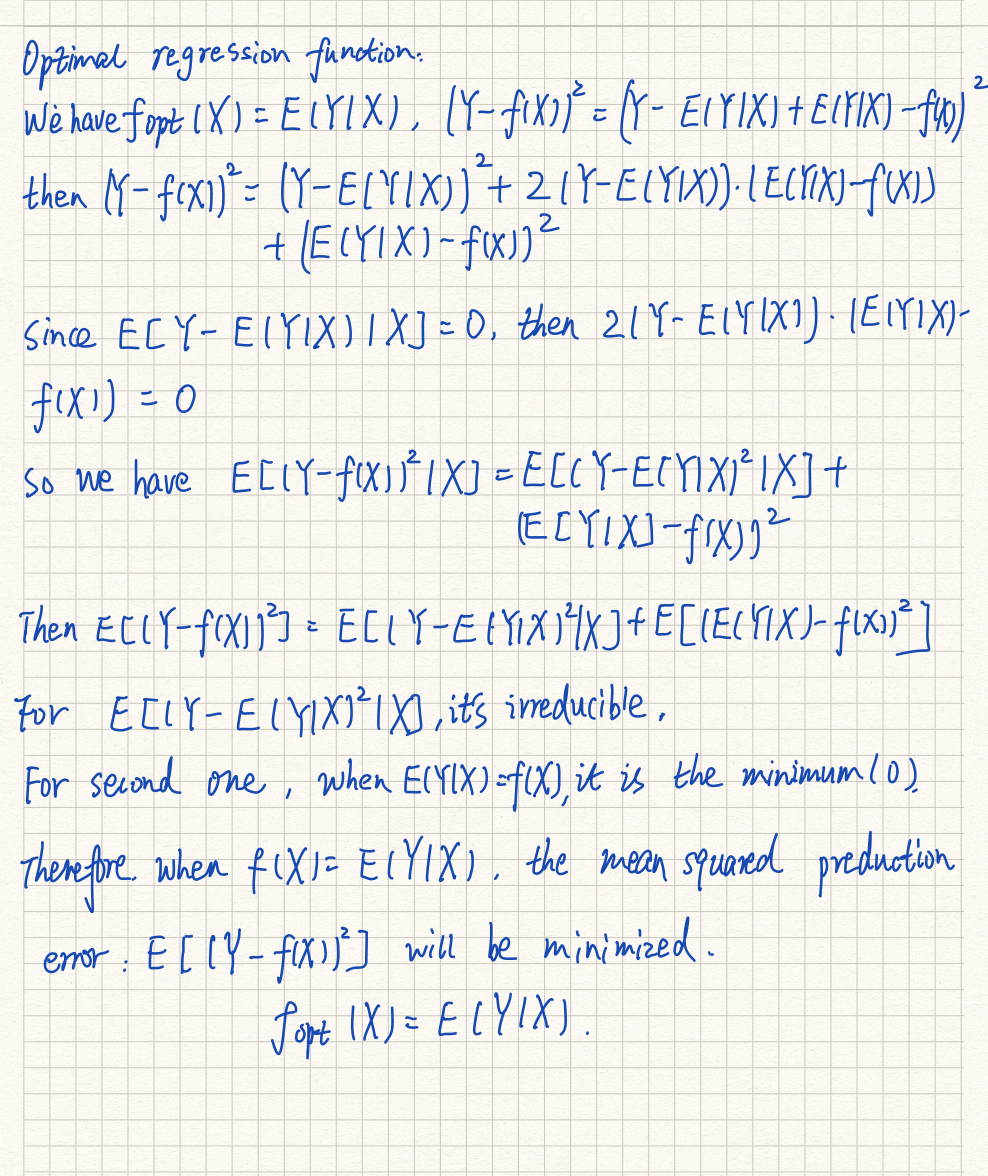
\includegraphics{images/clipboard-2780810541.jpeg}

Bias-variance trade-off:

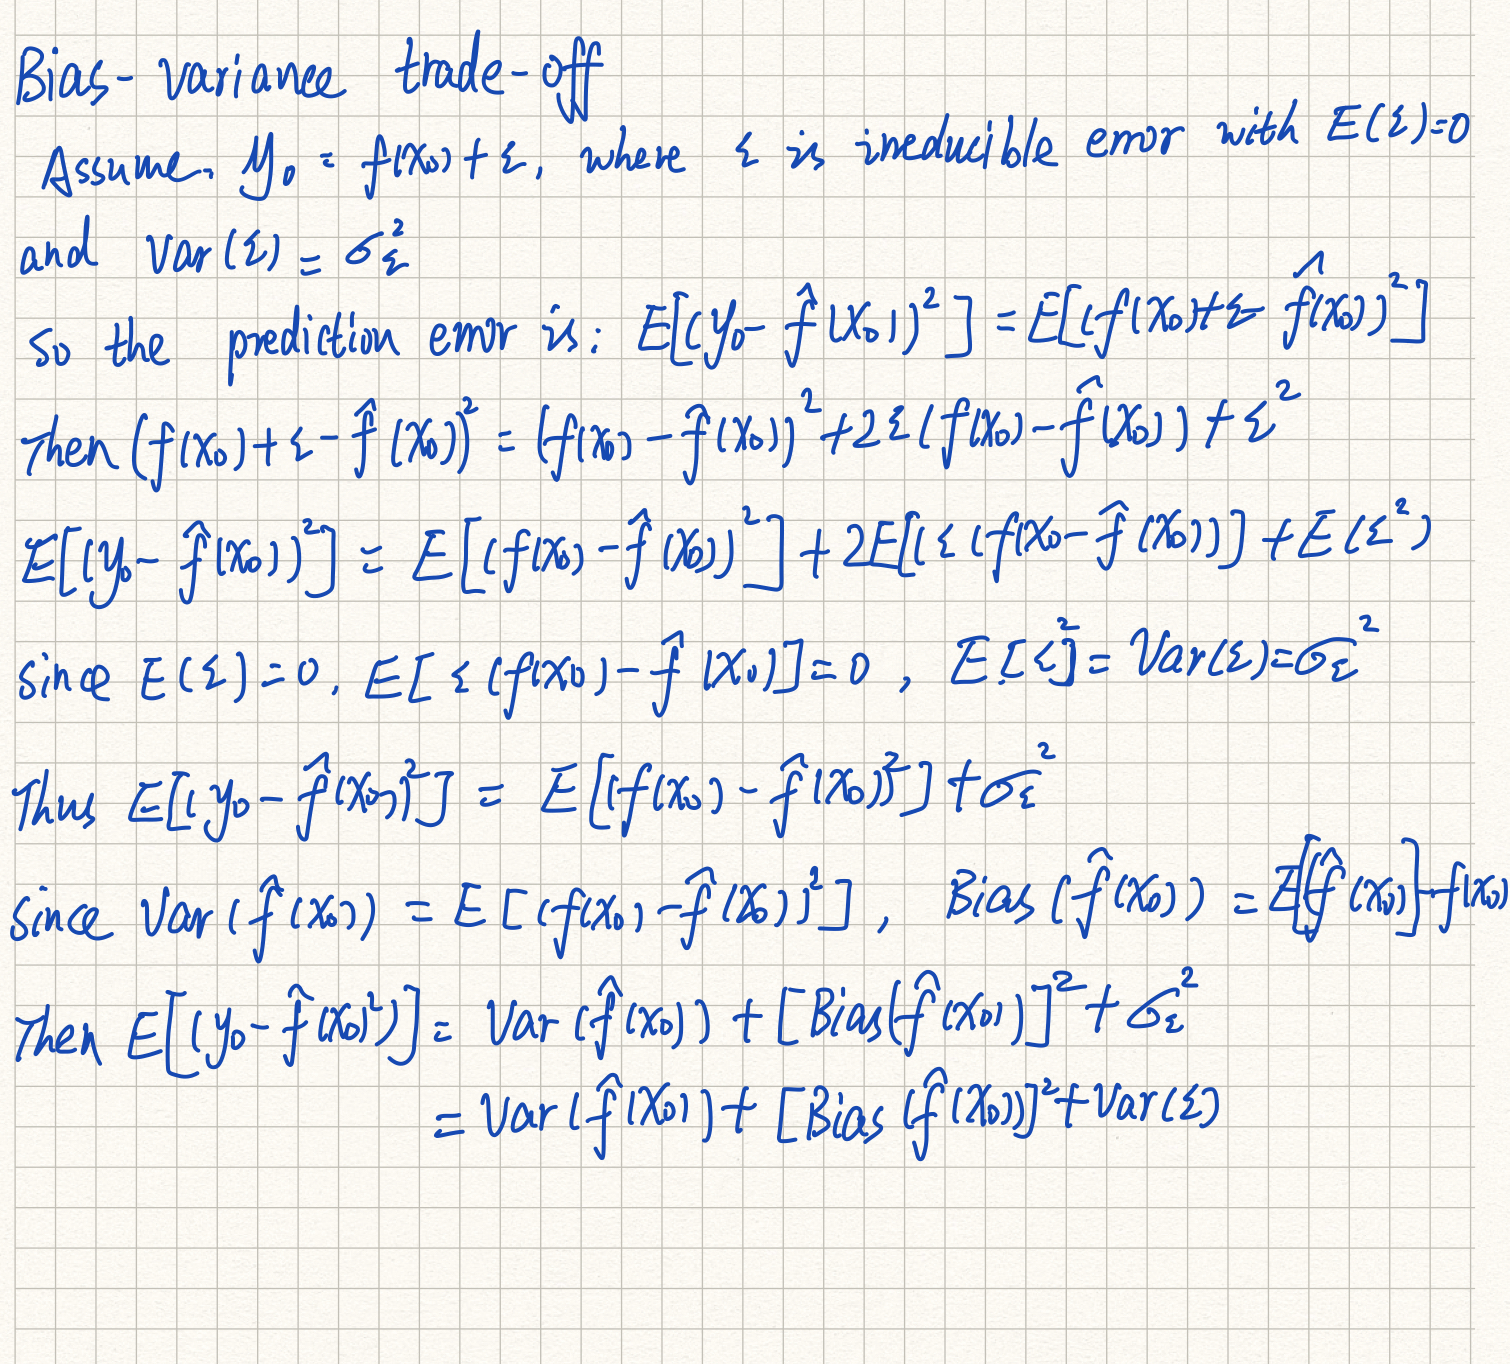
\includegraphics{images/clipboard-2041856251.jpeg}

\hypertarget{isl-exercise-2.4.3-10-pts}{%
\subsection{ISL Exercise 2.4.3 (10\%
pts)}\label{isl-exercise-2.4.3-10-pts}}

\begin{Shaded}
\begin{Highlighting}[]
\FunctionTok{library}\NormalTok{(tidyverse)}
\NormalTok{fit }\OtherTok{\textless{}{-}} \FunctionTok{lm}\NormalTok{(sales }\SpecialCharTok{\textasciitilde{}}\NormalTok{ TV, }\AttributeTok{data =}\NormalTok{ )}
\end{Highlighting}
\end{Shaded}

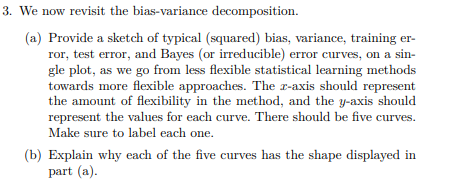
\includegraphics[width=5.48958in,height=\textheight]{images/clipboard-2321342665.png}

(a)

\begin{Shaded}
\begin{Highlighting}[]
\FunctionTok{library}\NormalTok{(ggplot2)}

\NormalTok{Flexibility }\OtherTok{\textless{}{-}} \DecValTok{1}\SpecialCharTok{:}\DecValTok{100}
\NormalTok{Bias }\OtherTok{\textless{}{-}} \DecValTok{100} \SpecialCharTok{/}\NormalTok{ Flexibility }
\NormalTok{Variance }\OtherTok{\textless{}{-}}\NormalTok{ Flexibility }\SpecialCharTok{/} \DecValTok{10} 
\NormalTok{TrainingError }\OtherTok{\textless{}{-}} \DecValTok{100} \SpecialCharTok{/}\NormalTok{ Flexibility}
\NormalTok{TestError }\OtherTok{\textless{}{-}}\NormalTok{ Bias }\SpecialCharTok{+}\NormalTok{ Variance }
\NormalTok{BayesError }\OtherTok{\textless{}{-}} \FunctionTok{rep}\NormalTok{(}\DecValTok{10}\NormalTok{, }\DecValTok{100}\NormalTok{)  }

\CommentTok{\# Combine into a data frame}
\NormalTok{data }\OtherTok{\textless{}{-}} \FunctionTok{data.frame}\NormalTok{(}
  \AttributeTok{Flexibility =}\NormalTok{ Flexibility,}
  \AttributeTok{Bias =}\NormalTok{ Bias,}
  \AttributeTok{Variance =}\NormalTok{ Variance,}
  \AttributeTok{TrainingError =}\NormalTok{ TrainingError,}
  \AttributeTok{TestError =}\NormalTok{ TestError,}
  \AttributeTok{BayesError =}\NormalTok{ BayesError}
\NormalTok{)}
\NormalTok{data\_long }\OtherTok{\textless{}{-}}\NormalTok{ reshape2}\SpecialCharTok{::}\FunctionTok{melt}\NormalTok{(data, }\AttributeTok{id.vars =} \StringTok{"Flexibility"}\NormalTok{, }\AttributeTok{variable.name =} \StringTok{"ErrorType"}\NormalTok{, }\AttributeTok{value.name =} \StringTok{"ErrorValue"}\NormalTok{)}

\FunctionTok{ggplot}\NormalTok{(data\_long, }\FunctionTok{aes}\NormalTok{(}\AttributeTok{x =}\NormalTok{ Flexibility, }\AttributeTok{y =}\NormalTok{ ErrorValue, }\AttributeTok{color =}\NormalTok{ ErrorType)) }\SpecialCharTok{+}
  \FunctionTok{geom\_line}\NormalTok{(}\AttributeTok{size =} \FloatTok{1.2}\NormalTok{) }\SpecialCharTok{+}
  \FunctionTok{labs}\NormalTok{(}
    \AttributeTok{title =} \StringTok{"Bias{-}Variance Decomposition"}\NormalTok{,}
    \AttributeTok{x =} \StringTok{"Model Flexibility"}\NormalTok{,}
    \AttributeTok{y =} \StringTok{"Error Value"}\NormalTok{,}
    \AttributeTok{color =} \StringTok{"Error Components"}
\NormalTok{  ) }\SpecialCharTok{+}
  \FunctionTok{scale\_color\_manual}\NormalTok{(}
    \AttributeTok{values =} \FunctionTok{c}\NormalTok{(}\StringTok{"blue"}\NormalTok{, }\StringTok{"red"}\NormalTok{, }\StringTok{"green"}\NormalTok{, }\StringTok{"purple"}\NormalTok{, }\StringTok{"orange"}\NormalTok{),}
    \AttributeTok{labels =} \FunctionTok{c}\NormalTok{(}\StringTok{"Bias (Squared)"}\NormalTok{, }\StringTok{"Variance"}\NormalTok{, }\StringTok{"Training Error"}\NormalTok{, }\StringTok{"Test Error"}\NormalTok{, }\StringTok{"Bayes Error"}\NormalTok{)}
\NormalTok{  ) }\SpecialCharTok{+}
  \FunctionTok{theme\_minimal}\NormalTok{() }\SpecialCharTok{+}
  \FunctionTok{theme}\NormalTok{(}
    \AttributeTok{legend.position =} \StringTok{"right"}\NormalTok{,}
    \AttributeTok{plot.title =} \FunctionTok{element\_text}\NormalTok{(}\AttributeTok{size =} \DecValTok{14}\NormalTok{, }\AttributeTok{face =} \StringTok{"bold"}\NormalTok{, }\AttributeTok{hjust =} \FloatTok{0.5}\NormalTok{)}
\NormalTok{  )}
\end{Highlighting}
\end{Shaded}

\begin{verbatim}
Warning: Using `size` aesthetic for lines was deprecated in ggplot2 3.4.0.
i Please use `linewidth` instead.
\end{verbatim}

\begin{figure}[H]

{\centering 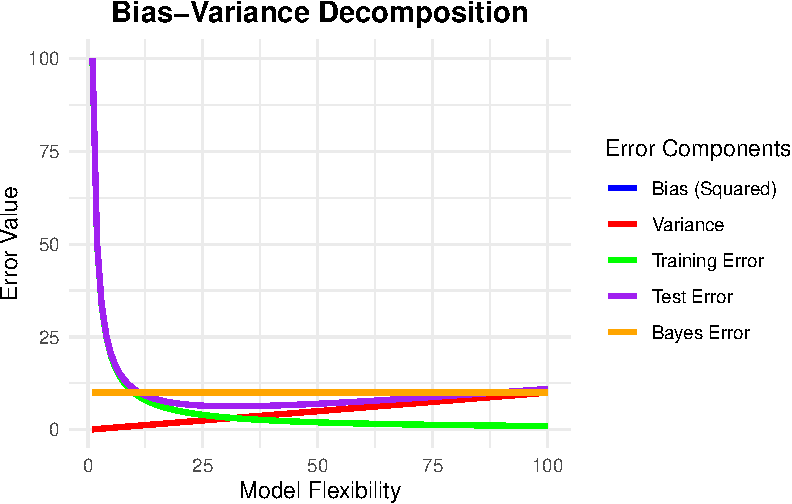
\includegraphics{hw1_files/figure-pdf/unnamed-chunk-2-1.pdf}

}

\end{figure}

(b) Bias Curve: Decreases because as flexibility increases, the model
can better fit the training data, reducing systematic error.Variance
Curve: Increases because more flexible models are more sensitive to
small fluctuations in the data, leading to overfitting.Training Error
Curve: Always decreases because more flexible models can perfectly fit
(or nearly fit) the training data.Test Error Curve: U-shaped because it
is influenced by both bias and variance. Initially, test error decreases
as bias dominates. Later, it increases as variance dominates.Bayes
Error: Stays constant as it represents noise or irreducible error in the
data.

\hypertarget{isl-exercise-2.4.4-10-pts}{%
\subsection{ISL Exercise 2.4.4 (10\%
pts)}\label{isl-exercise-2.4.4-10-pts}}

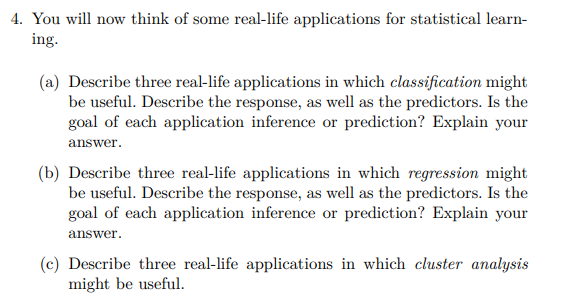
\includegraphics{images/clipboard-1845645679.png}

(a) Classification application:

Spam email detection: Response: Email is spam (1) or not (0).
Predictors: Frequency of certain keywords, length of the email, etc.
Goal: Prediction. The model is used to predict whether new emails are
spam or not.

Medical Diagnosis: Response: Whether a patient has a disease Yes (1) or
not (0).

Predictors: Age, gender, symptoms, test results, and medical history.
Goal: Inference and prediction. Inference is used to understand which
predictors are most associated with the disease. Prediction is used to
diagnose new patients.

Disease classification: Response variable: the disease classification of
the patient, such as diabetes (1) , heart disease (2) , health (0) .
Predictive variables: age, blood glucose level, cholesterol level,
medical history, lifestyle, etc. Goal: Predict. Assist doctors in making
quick diagnostic decisions.

(b) Regression application:

Drug dosage and efficacy: Response: Drug efficacy (such as decreased
blood glucose levels). Predictive : drug dosage, patient age, weight,
etc. Goal: Inference. Assist in drug research, analyze the relationship
between dosage and efficacy.

Real estate rent forecast:Response : Rent price. Predictive :
geographical location, area, decoration level, surrounding facilities,
etc. Goal: Predict. Provide reference prices for the rental market.

Stock market analysis:Response: Future stock price or return. Predictive
: historical prices, trading volume, economic indicators, and news
sentiment. Goal: Predict. This model helps predict stock prices for
investment decisions.

(c) Cluster application:

Grouping students based on their academic performance and learning
behavior. Features: classroom performance, exam scores, participation,
completion of assignments, etc. Goal: To assist teachers in developing
teaching plans for different groups. Genotyping analysis

Grouping genes based on DNA sequence data. Features: gene expression
level, sequence similarity, etc. Goal: To discover different types of
genomic populations for disease research. Retail store location
selection

Grouping urban areas based on population density and consumption
behavior. Features: Population characteristics (age, income), traffic
flow, consumption level, etc. Goal: Help retailers choose the best
location.

\hypertarget{isl-exercise-2.4.10-30-pts}{%
\subsection{ISL Exercise 2.4.10 (30\%
pts)}\label{isl-exercise-2.4.10-30-pts}}

Your can read in the \texttt{boston} data set directly from url
\url{https://raw.githubusercontent.com/ucla-biostat-212a/2024winter/master/slides/data/Boston.csv}.
A documentation of the \texttt{boston} data set is
\href{https://www.rdocumentation.org/packages/ISLR2/versions/1.3-2/topics/Boston}{here}.

\paragraph{R}

\begin{Shaded}
\begin{Highlighting}[]
\FunctionTok{library}\NormalTok{(tidyverse)}
\NormalTok{Boston }\OtherTok{\textless{}{-}} \FunctionTok{read\_csv}\NormalTok{(}\StringTok{"https://raw.githubusercontent.com/ucla{-}biostat{-}212a/2024winter/master/slides/data/Boston.csv"}\NormalTok{, }\AttributeTok{col\_select =} \SpecialCharTok{{-}}\DecValTok{1}\NormalTok{) }\SpecialCharTok{\%\textgreater{}\%} 
  \FunctionTok{print}\NormalTok{(}\AttributeTok{width =} \ConstantTok{Inf}\NormalTok{)}
\end{Highlighting}
\end{Shaded}

\begin{verbatim}
# A tibble: 506 x 13
      crim    zn indus  chas   nox    rm   age   dis   rad   tax ptratio lstat
     <dbl> <dbl> <dbl> <dbl> <dbl> <dbl> <dbl> <dbl> <dbl> <dbl>   <dbl> <dbl>
 1 0.00632  18    2.31     0 0.538  6.58  65.2  4.09     1   296    15.3  4.98
 2 0.0273    0    7.07     0 0.469  6.42  78.9  4.97     2   242    17.8  9.14
 3 0.0273    0    7.07     0 0.469  7.18  61.1  4.97     2   242    17.8  4.03
 4 0.0324    0    2.18     0 0.458  7.00  45.8  6.06     3   222    18.7  2.94
 5 0.0690    0    2.18     0 0.458  7.15  54.2  6.06     3   222    18.7  5.33
 6 0.0298    0    2.18     0 0.458  6.43  58.7  6.06     3   222    18.7  5.21
 7 0.0883   12.5  7.87     0 0.524  6.01  66.6  5.56     5   311    15.2 12.4 
 8 0.145    12.5  7.87     0 0.524  6.17  96.1  5.95     5   311    15.2 19.2 
 9 0.211    12.5  7.87     0 0.524  5.63 100    6.08     5   311    15.2 29.9 
10 0.170    12.5  7.87     0 0.524  6.00  85.9  6.59     5   311    15.2 17.1 
    medv
   <dbl>
 1  24  
 2  21.6
 3  34.7
 4  33.4
 5  36.2
 6  28.7
 7  22.9
 8  27.1
 9  16.5
10  18.9
# i 496 more rows
\end{verbatim}

\paragraph{Python}

\begin{Shaded}
\begin{Highlighting}[]
\CommentTok{\# import pandas as pd}
\CommentTok{\# import io}
\CommentTok{\# import requests}
\CommentTok{\# }
\CommentTok{\# url = "https://raw.githubusercontent.com/ucla{-}econ{-}425t/2023winter/master/slides/data/Boston.csv"}
\CommentTok{\# s = requests.get(url).content}
\CommentTok{\# Boston = pd.read\_csv(io.StringIO(s.decode(\textquotesingle{}utf{-}8\textquotesingle{})), index\_col = 0)}
\CommentTok{\# Boston}
\end{Highlighting}
\end{Shaded}

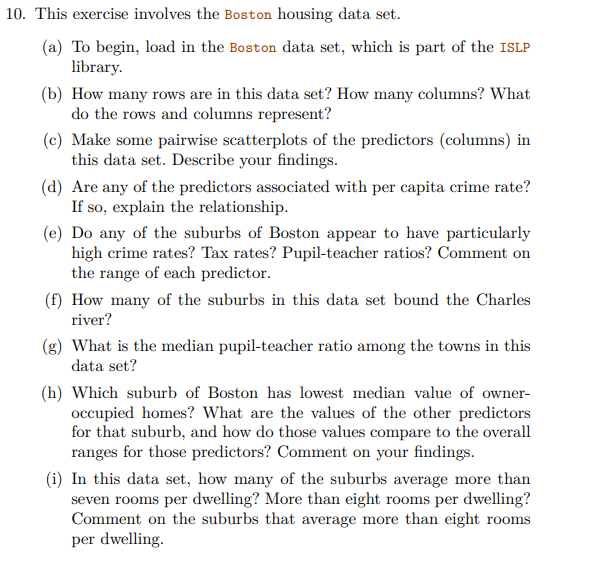
\includegraphics{images/clipboard-2802351124.png}

(a)

\begin{Shaded}
\begin{Highlighting}[]
\FunctionTok{library}\NormalTok{(tidyverse)}
\NormalTok{Boston }\OtherTok{\textless{}{-}} \FunctionTok{read\_csv}\NormalTok{(}\StringTok{"https://raw.githubusercontent.com/ucla{-}biostat{-}212a/2024winter/master/slides/data/Boston.csv"}\NormalTok{, }\AttributeTok{col\_select =} \SpecialCharTok{{-}}\DecValTok{1}\NormalTok{) }\SpecialCharTok{\%\textgreater{}\%} 
  \FunctionTok{print}\NormalTok{(}\AttributeTok{width =} \ConstantTok{Inf}\NormalTok{)}
\end{Highlighting}
\end{Shaded}

\begin{verbatim}
# A tibble: 506 x 13
      crim    zn indus  chas   nox    rm   age   dis   rad   tax ptratio lstat
     <dbl> <dbl> <dbl> <dbl> <dbl> <dbl> <dbl> <dbl> <dbl> <dbl>   <dbl> <dbl>
 1 0.00632  18    2.31     0 0.538  6.58  65.2  4.09     1   296    15.3  4.98
 2 0.0273    0    7.07     0 0.469  6.42  78.9  4.97     2   242    17.8  9.14
 3 0.0273    0    7.07     0 0.469  7.18  61.1  4.97     2   242    17.8  4.03
 4 0.0324    0    2.18     0 0.458  7.00  45.8  6.06     3   222    18.7  2.94
 5 0.0690    0    2.18     0 0.458  7.15  54.2  6.06     3   222    18.7  5.33
 6 0.0298    0    2.18     0 0.458  6.43  58.7  6.06     3   222    18.7  5.21
 7 0.0883   12.5  7.87     0 0.524  6.01  66.6  5.56     5   311    15.2 12.4 
 8 0.145    12.5  7.87     0 0.524  6.17  96.1  5.95     5   311    15.2 19.2 
 9 0.211    12.5  7.87     0 0.524  5.63 100    6.08     5   311    15.2 29.9 
10 0.170    12.5  7.87     0 0.524  6.00  85.9  6.59     5   311    15.2 17.1 
    medv
   <dbl>
 1  24  
 2  21.6
 3  34.7
 4  33.4
 5  36.2
 6  28.7
 7  22.9
 8  27.1
 9  16.5
10  18.9
# i 496 more rows
\end{verbatim}

Done!\\
(b)

\begin{Shaded}
\begin{Highlighting}[]
\FunctionTok{nrow}\NormalTok{(Boston)  }
\end{Highlighting}
\end{Shaded}

\begin{verbatim}
[1] 506
\end{verbatim}

\begin{Shaded}
\begin{Highlighting}[]
\FunctionTok{ncol}\NormalTok{(Boston)  }
\end{Highlighting}
\end{Shaded}

\begin{verbatim}
[1] 13
\end{verbatim}

There are 506 rows and 13 columns. Rows represent suburbs or towns in
the Boston area. Each column represents a feature or response variable
(e.g., crime rate, tax rate, median value of homes).

(c)

\begin{Shaded}
\begin{Highlighting}[]
\FunctionTok{library}\NormalTok{(ISLR2)}
\FunctionTok{library}\NormalTok{(GGally)}
\FunctionTok{library}\NormalTok{(ggplot2)}
\FunctionTok{ggpairs}\NormalTok{(}
  \AttributeTok{data =}\NormalTok{ Boston,  }
  \AttributeTok{mapping =} \FunctionTok{aes}\NormalTok{(}\AttributeTok{alpha =} \FloatTok{0.5}\NormalTok{),}
  \AttributeTok{upper =} \FunctionTok{list}\NormalTok{(}\AttributeTok{continuous =} \FunctionTok{wrap}\NormalTok{(}\StringTok{"cor"}\NormalTok{, }\AttributeTok{size =} \DecValTok{3}\NormalTok{)), }
  \AttributeTok{lower =} \FunctionTok{list}\NormalTok{(}\AttributeTok{continuous =} \FunctionTok{wrap}\NormalTok{(}\StringTok{"smooth"}\NormalTok{, }\AttributeTok{method =} \StringTok{"lm"}\NormalTok{, }\AttributeTok{se =} \ConstantTok{FALSE}\NormalTok{))}
\NormalTok{) }\SpecialCharTok{+} 
  \FunctionTok{labs}\NormalTok{(}\AttributeTok{title =} \StringTok{"Pairwise Scatterplots of All Predictors"}\NormalTok{)}
\end{Highlighting}
\end{Shaded}

\begin{figure}[H]

{\centering 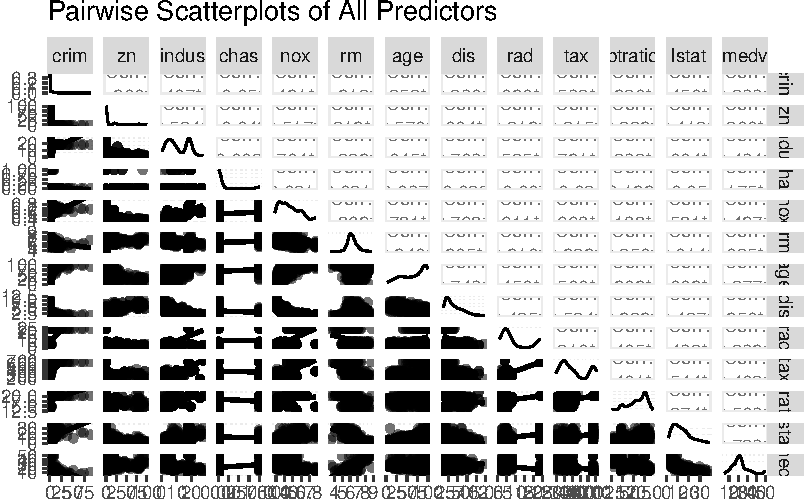
\includegraphics{hw1_files/figure-pdf/unnamed-chunk-7-1.pdf}

}

\end{figure}

The correlation coefficient between Zn and Crimea is -0.200, showing a
weak negative correlation. When Zn increases, there is a slight downward
trend in Crimea.Indus is moderately positively correlated with Crimea. A
higher proportion of industrial land is associated with a higher crime
rate.chas: The correlation coefficient with Crimea is -0.056, indicating
no significant linear relationship.The correlation coefficient between
NOx and Crimea is 0.421, showing a moderate positive correlation. Higher
concentrations of nitric oxide may be associated with higher crime
rates.rm: The correlation coefficient with Crimea is -0.219, showing a
weak negative correlation. The crime rate is higher when the average
number of rooms is small.

The correlation coefficient between Indus and NOx is 0.764, showing a
strong positive correlation, indicating that the higher the proportion
of industrial land, the more severe the air pollution (NOx).RM is
negatively correlated with both Indus and NOX, indicating that houses
with more rooms are usually located in areas with lower industrial land
ratios and less pollution.Distribution shape and pattern:Some variables,
such as zn and crim, exhibit nonlinear patterns and may require further
exploration of their nonlinear relationships.

(d)

\begin{Shaded}
\begin{Highlighting}[]
\FunctionTok{library}\NormalTok{(MASS)}
\FunctionTok{data}\NormalTok{(Boston)}
\NormalTok{results }\OtherTok{\textless{}{-}} \FunctionTok{data.frame}\NormalTok{(}\AttributeTok{Predictor =} \FunctionTok{character}\NormalTok{(), }\AttributeTok{Coefficient =} \FunctionTok{numeric}\NormalTok{(), }\AttributeTok{P\_Value =} \FunctionTok{numeric}\NormalTok{())}
\ControlFlowTok{for}\NormalTok{ (predictor }\ControlFlowTok{in} \FunctionTok{colnames}\NormalTok{(Boston)[}\SpecialCharTok{{-}}\DecValTok{1}\NormalTok{]) \{  }\CommentTok{\# Exclude \textasciigrave{}crim\textasciigrave{} as it\textquotesingle{}s the response variable}
\NormalTok{  model }\OtherTok{\textless{}{-}} \FunctionTok{lm}\NormalTok{(crim }\SpecialCharTok{\textasciitilde{}}\NormalTok{ Boston[[predictor]], }\AttributeTok{data =}\NormalTok{ Boston)}
\NormalTok{  summary\_model }\OtherTok{\textless{}{-}} \FunctionTok{summary}\NormalTok{(model)}
\NormalTok{  results }\OtherTok{\textless{}{-}} \FunctionTok{rbind}\NormalTok{(results, }\FunctionTok{data.frame}\NormalTok{(}
    \AttributeTok{Predictor =}\NormalTok{ predictor,}
    \AttributeTok{Coefficient =} \FunctionTok{coef}\NormalTok{(summary\_model)[}\DecValTok{2}\NormalTok{, }\DecValTok{1}\NormalTok{],  }\CommentTok{\# Slope (relationship strength and direction)}
    \AttributeTok{P\_Value =} \FunctionTok{coef}\NormalTok{(summary\_model)[}\DecValTok{2}\NormalTok{, }\DecValTok{4}\NormalTok{]      }\CommentTok{\# P{-}value (significance)}
\NormalTok{  ))}
\NormalTok{\}}

\NormalTok{significant\_results }\OtherTok{\textless{}{-}} \FunctionTok{subset}\NormalTok{(results, P\_Value }\SpecialCharTok{\textless{}} \FloatTok{0.05}\NormalTok{)}
\FunctionTok{print}\NormalTok{(}\StringTok{"Significant Predictors Associated with Crime Rate:"}\NormalTok{)}
\end{Highlighting}
\end{Shaded}

\begin{verbatim}
[1] "Significant Predictors Associated with Crime Rate:"
\end{verbatim}

\begin{Shaded}
\begin{Highlighting}[]
\FunctionTok{print}\NormalTok{(significant\_results)}
\end{Highlighting}
\end{Shaded}

\begin{verbatim}
   Predictor Coefficient      P_Value
1         zn -0.07393498 5.506472e-06
2      indus  0.50977633 1.450349e-21
4        nox 31.24853120 3.751739e-23
5         rm -2.68405122 6.346703e-07
6        age  0.10778623 2.854869e-16
7        dis -1.55090168 8.519949e-19
8        rad  0.61791093 2.693844e-56
9        tax  0.02974225 2.357127e-47
10   ptratio  1.15198279 2.942922e-11
11     black -0.03627964 2.487274e-19
12     lstat  0.54880478 2.654277e-27
13      medv -0.36315992 1.173987e-19
\end{verbatim}

The crime rate is significantly positively correlated with factors such
as the industrial land ratio (indus), nitric oxide concentration (NOx),
age of old houses, highway accessibility (rad), property tax rate (tax),
and student teacher ratio (ptratio). This indicates that areas with high
levels of economic industrialization, severe air pollution, convenient
transportation, but limited educational resources have higher crime
rates.

The crime rate is significantly negatively correlated with the
proportion of large-scale residential land (Zn), the average number of
rooms in a house (RM), the weighted distance from the employment center
(DIS), and the proportion of black people (Black). These results
indicate that low-density residential communities, higher housing
quality, areas further away from urban employment centers, and areas
with a higher proportion of black people have lower crime rates.

(e)

\begin{Shaded}
\begin{Highlighting}[]
\FunctionTok{summary}\NormalTok{(Boston}\SpecialCharTok{$}\NormalTok{crim)}
\end{Highlighting}
\end{Shaded}

\begin{verbatim}
    Min.  1st Qu.   Median     Mean  3rd Qu.     Max. 
 0.00632  0.08204  0.25651  3.61352  3.67708 88.97620 
\end{verbatim}

\begin{Shaded}
\begin{Highlighting}[]
\FunctionTok{summary}\NormalTok{(Boston}\SpecialCharTok{$}\NormalTok{tax)}
\end{Highlighting}
\end{Shaded}

\begin{verbatim}
   Min. 1st Qu.  Median    Mean 3rd Qu.    Max. 
  187.0   279.0   330.0   408.2   666.0   711.0 
\end{verbatim}

\begin{Shaded}
\begin{Highlighting}[]
\FunctionTok{summary}\NormalTok{(Boston}\SpecialCharTok{$}\NormalTok{ptratio)}
\end{Highlighting}
\end{Shaded}

\begin{verbatim}
   Min. 1st Qu.  Median    Mean 3rd Qu.    Max. 
  12.60   17.40   19.05   18.46   20.20   22.00 
\end{verbatim}

\begin{Shaded}
\begin{Highlighting}[]
\NormalTok{high\_crime }\OtherTok{\textless{}{-}}\NormalTok{ Boston[Boston}\SpecialCharTok{$}\NormalTok{crim }\SpecialCharTok{\textgreater{}} \FunctionTok{quantile}\NormalTok{(Boston}\SpecialCharTok{$}\NormalTok{crim, }\FloatTok{0.8}\NormalTok{), ]}
\NormalTok{high\_tax }\OtherTok{\textless{}{-}}\NormalTok{ Boston[Boston}\SpecialCharTok{$}\NormalTok{tax }\SpecialCharTok{\textgreater{}} \FunctionTok{quantile}\NormalTok{(Boston}\SpecialCharTok{$}\NormalTok{tax, }\FloatTok{0.8}\NormalTok{), ]}
\NormalTok{high\_ptratio }\OtherTok{\textless{}{-}}\NormalTok{ Boston[Boston}\SpecialCharTok{$}\NormalTok{ptratio }\SpecialCharTok{\textgreater{}} \FunctionTok{quantile}\NormalTok{(Boston}\SpecialCharTok{$}\NormalTok{ptratio, }\FloatTok{0.8}\NormalTok{), ]}
 
\FunctionTok{cat}\NormalTok{(}\StringTok{"High Crime:"}\NormalTok{, }\FunctionTok{nrow}\NormalTok{(high\_crime), }
    \StringTok{"}\SpecialCharTok{\textbackslash{}n}\StringTok{High Tax:"}\NormalTok{, }\FunctionTok{nrow}\NormalTok{(high\_tax), }
    \StringTok{"}\SpecialCharTok{\textbackslash{}n}\StringTok{High Pupil{-}Teacher Ratio:"}\NormalTok{, }\FunctionTok{nrow}\NormalTok{(high\_ptratio), }\StringTok{"}\SpecialCharTok{\textbackslash{}n}\StringTok{"}\NormalTok{)}
\end{Highlighting}
\end{Shaded}

\begin{verbatim}
High Crime: 101 
High Tax: 5 
High Pupil-Teacher Ratio: 56 
\end{verbatim}

The distribution of crime rates is extremely uneven, with some suburban
areas (such as crime rates\textgreater3.67708) being high crime areas,
with the highest values far above the average, and there are obvious
extreme values (such as the highest value of 88.97620).

The tax rate distribution is relatively concentrated, with most suburbs
having tax rates ranging from 187 to 666, and only a few suburbs (such
as\textgreater666) at high tax rates.

The distribution of student teacher ratio is relatively even, with only
some suburban areas experiencing significant shortage of educational
resources (e.g.\textgreater20)

(f)

\begin{Shaded}
\begin{Highlighting}[]
\FunctionTok{sum}\NormalTok{(Boston}\SpecialCharTok{$}\NormalTok{chas }\SpecialCharTok{==} \DecValTok{1}\NormalTok{)  }
\end{Highlighting}
\end{Shaded}

\begin{verbatim}
[1] 35
\end{verbatim}

There are 35 suburbs bound the Charles river.

(g)

\begin{Shaded}
\begin{Highlighting}[]
\FunctionTok{median}\NormalTok{(Boston}\SpecialCharTok{$}\NormalTok{ptratio, }\AttributeTok{na.rm =} \ConstantTok{TRUE}\NormalTok{)}
\end{Highlighting}
\end{Shaded}

\begin{verbatim}
[1] 19.05
\end{verbatim}

The median pupil-teacher ratio among the towns is 19.05.

(h)

\begin{Shaded}
\begin{Highlighting}[]
\NormalTok{lowest\_medv }\OtherTok{\textless{}{-}}\NormalTok{ Boston[}\FunctionTok{which.min}\NormalTok{(Boston}\SpecialCharTok{$}\NormalTok{medv), ]}
\NormalTok{lowest\_medv}
\end{Highlighting}
\end{Shaded}

\begin{verbatim}
       crim zn indus chas   nox    rm age    dis rad tax ptratio black lstat
399 38.3518  0  18.1    0 0.693 5.453 100 1.4896  24 666    20.2 396.9 30.59
    medv
399    5
\end{verbatim}

The high crime rate is an important factor in the decline of housing
prices.A high proportion of old buildings may reduce their
attractiveness.Severe air pollution and high level of industrialization:
have a negative impact on the quality of living environment.High tax
rates and limited educational resources will increase the cost of living
and reduce the attractiveness of housing.

(i)

\begin{Shaded}
\begin{Highlighting}[]
\NormalTok{over\_7\_rooms }\OtherTok{\textless{}{-}} \FunctionTok{sum}\NormalTok{(Boston}\SpecialCharTok{$}\NormalTok{rm }\SpecialCharTok{\textgreater{}} \DecValTok{7}\NormalTok{)}
\NormalTok{over\_8\_rooms }\OtherTok{\textless{}{-}} \FunctionTok{sum}\NormalTok{(Boston}\SpecialCharTok{$}\NormalTok{rm }\SpecialCharTok{\textgreater{}} \DecValTok{8}\NormalTok{)}

\NormalTok{over\_7\_rooms}
\end{Highlighting}
\end{Shaded}

\begin{verbatim}
[1] 64
\end{verbatim}

\begin{Shaded}
\begin{Highlighting}[]
\NormalTok{over\_8\_rooms}
\end{Highlighting}
\end{Shaded}

\begin{verbatim}
[1] 13
\end{verbatim}

\begin{Shaded}
\begin{Highlighting}[]
\NormalTok{Boston[Boston}\SpecialCharTok{$}\NormalTok{rm }\SpecialCharTok{\textgreater{}} \DecValTok{8}\NormalTok{, ]}
\end{Highlighting}
\end{Shaded}

\begin{verbatim}
       crim zn indus chas    nox    rm  age    dis rad tax ptratio  black lstat
98  0.12083  0  2.89    0 0.4450 8.069 76.0 3.4952   2 276    18.0 396.90  4.21
164 1.51902  0 19.58    1 0.6050 8.375 93.9 2.1620   5 403    14.7 388.45  3.32
205 0.02009 95  2.68    0 0.4161 8.034 31.9 5.1180   4 224    14.7 390.55  2.88
225 0.31533  0  6.20    0 0.5040 8.266 78.3 2.8944   8 307    17.4 385.05  4.14
226 0.52693  0  6.20    0 0.5040 8.725 83.0 2.8944   8 307    17.4 382.00  4.63
227 0.38214  0  6.20    0 0.5040 8.040 86.5 3.2157   8 307    17.4 387.38  3.13
233 0.57529  0  6.20    0 0.5070 8.337 73.3 3.8384   8 307    17.4 385.91  2.47
234 0.33147  0  6.20    0 0.5070 8.247 70.4 3.6519   8 307    17.4 378.95  3.95
254 0.36894 22  5.86    0 0.4310 8.259  8.4 8.9067   7 330    19.1 396.90  3.54
258 0.61154 20  3.97    0 0.6470 8.704 86.9 1.8010   5 264    13.0 389.70  5.12
263 0.52014 20  3.97    0 0.6470 8.398 91.5 2.2885   5 264    13.0 386.86  5.91
268 0.57834 20  3.97    0 0.5750 8.297 67.0 2.4216   5 264    13.0 384.54  7.44
365 3.47428  0 18.10    1 0.7180 8.780 82.9 1.9047  24 666    20.2 354.55  5.29
    medv
98  38.7
164 50.0
205 50.0
225 44.8
226 50.0
227 37.6
233 41.7
234 48.3
254 42.8
258 50.0
263 48.8
268 50.0
365 21.9
\end{verbatim}

There are 64 and 13 suburbs average more than seven and eight rooms per
dwelling.

The crime rate in most suburbs is very low, with a minimum of 0.01208.
Some suburbs have a high proportion of large residential areas (such as
the suburbs with a Zn of 95). The lower concentration of nitric oxide
indicates lower air pollution in these areas (such as NOx mostly ranging
from 0.4 to 0.6). The proportion of house updates is relatively low in
some areas, such as some suburban areas with an age of less than 20.
These suburbs are often far from employment centers, indicating that
their locations are more remote.

\hypertarget{isl-exercise-3.7.3-20-pts}{%
\subsection{ISL Exercise 3.7.3 (20\%
pts)}\label{isl-exercise-3.7.3-20-pts}}

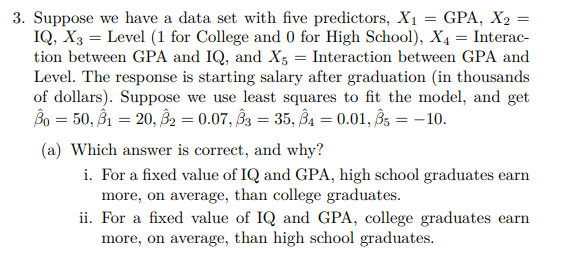
\includegraphics{images/clipboard-2573688108.png}

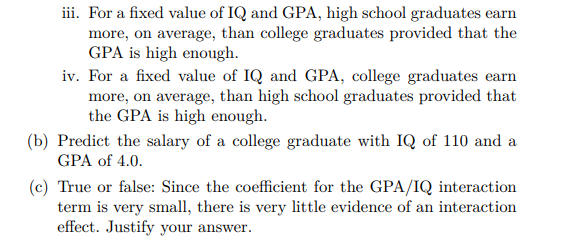
\includegraphics{images/clipboard-1304642707.png}

(a)-(b)

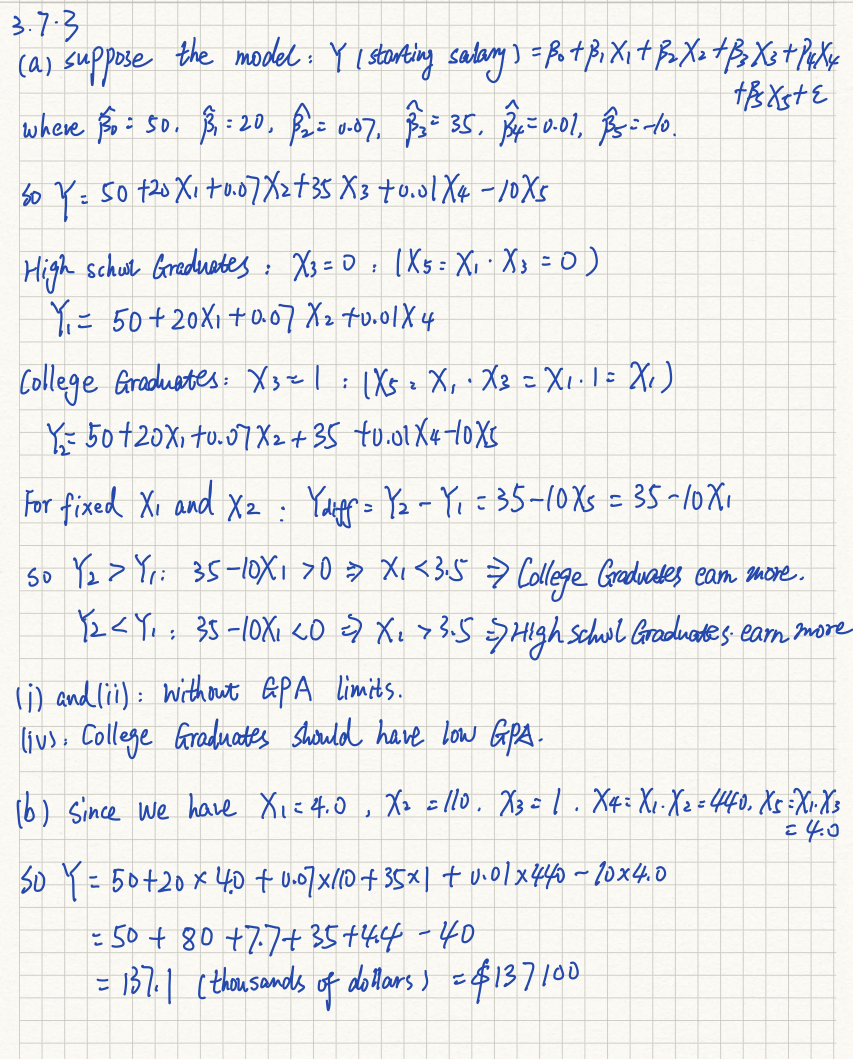
\includegraphics{images/17356e791ba29f6f2b80e5588c3b407.jpg}

(c) True. The coefficient for the GPA/IQ interaction term is very small,
suggesting that the interaction effect is minimal. The contribution of
\(\hatβ X​4\) =0.01⋅640=6.4, which is relatively small compared to other
terms.

\hypertarget{pts}{%
\subsection{3.7.15 (20\% pts)}\label{pts}}

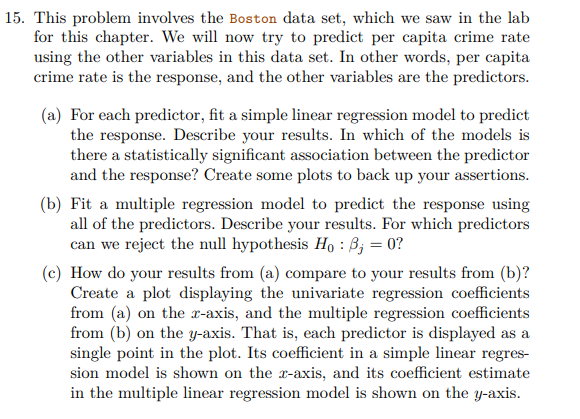
\includegraphics{images/clipboard-3010492794.png}

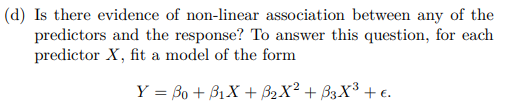
\includegraphics{images/clipboard-3808075512.png}

(a)

\begin{Shaded}
\begin{Highlighting}[]
\FunctionTok{library}\NormalTok{(MASS)}
\FunctionTok{data}\NormalTok{(Boston)}

\NormalTok{simple\_reg\_results }\OtherTok{\textless{}{-}} \FunctionTok{data.frame}\NormalTok{(}\AttributeTok{Predictor =} \FunctionTok{character}\NormalTok{(), }\AttributeTok{Coefficient =} \FunctionTok{numeric}\NormalTok{(), }\AttributeTok{P\_Value =} \FunctionTok{numeric}\NormalTok{())}

\ControlFlowTok{for}\NormalTok{ (predictor }\ControlFlowTok{in} \FunctionTok{colnames}\NormalTok{(Boston)[}\SpecialCharTok{{-}}\DecValTok{1}\NormalTok{]) \{}
\NormalTok{  model }\OtherTok{\textless{}{-}} \FunctionTok{lm}\NormalTok{(crim }\SpecialCharTok{\textasciitilde{}}\NormalTok{ Boston[[predictor]], }\AttributeTok{data =}\NormalTok{ Boston)}
\NormalTok{  summary\_model }\OtherTok{\textless{}{-}} \FunctionTok{summary}\NormalTok{(model)}
\NormalTok{  simple\_reg\_results }\OtherTok{\textless{}{-}} \FunctionTok{rbind}\NormalTok{(simple\_reg\_results, }\FunctionTok{data.frame}\NormalTok{(}
    \AttributeTok{Predictor =}\NormalTok{ predictor,}
    \AttributeTok{Coefficient =} \FunctionTok{coef}\NormalTok{(summary\_model)[}\DecValTok{2}\NormalTok{, }\DecValTok{1}\NormalTok{],}
    \AttributeTok{P\_Value =} \FunctionTok{coef}\NormalTok{(summary\_model)[}\DecValTok{2}\NormalTok{, }\DecValTok{4}\NormalTok{]}
\NormalTok{  ))}
\NormalTok{\}}

\NormalTok{significant\_predictors }\OtherTok{\textless{}{-}} \FunctionTok{subset}\NormalTok{(simple\_reg\_results, P\_Value }\SpecialCharTok{\textless{}} \FloatTok{0.05}\NormalTok{)}
\FunctionTok{print}\NormalTok{(significant\_predictors)}
\end{Highlighting}
\end{Shaded}

\begin{verbatim}
   Predictor Coefficient      P_Value
1         zn -0.07393498 5.506472e-06
2      indus  0.50977633 1.450349e-21
4        nox 31.24853120 3.751739e-23
5         rm -2.68405122 6.346703e-07
6        age  0.10778623 2.854869e-16
7        dis -1.55090168 8.519949e-19
8        rad  0.61791093 2.693844e-56
9        tax  0.02974225 2.357127e-47
10   ptratio  1.15198279 2.942922e-11
11     black -0.03627964 2.487274e-19
12     lstat  0.54880478 2.654277e-27
13      medv -0.36315992 1.173987e-19
\end{verbatim}

\begin{Shaded}
\begin{Highlighting}[]
\FunctionTok{library}\NormalTok{(ggplot2)}
\NormalTok{output\_folder }\OtherTok{\textless{}{-}} \StringTok{"crim\_plots"}
\ControlFlowTok{if}\NormalTok{ (}\SpecialCharTok{!}\FunctionTok{dir.exists}\NormalTok{(output\_folder)) \{}
  \FunctionTok{dir.create}\NormalTok{(output\_folder)}
\NormalTok{\}}

\ControlFlowTok{for}\NormalTok{ (predictor }\ControlFlowTok{in}\NormalTok{ significant\_predictors}\SpecialCharTok{$}\NormalTok{Predictor) \{}
\NormalTok{  p }\OtherTok{\textless{}{-}} \FunctionTok{ggplot}\NormalTok{(Boston, }\FunctionTok{aes}\NormalTok{(}\AttributeTok{x =}\NormalTok{ .data[[predictor]], }\AttributeTok{y =}\NormalTok{ crim)) }\SpecialCharTok{+}
    \FunctionTok{geom\_point}\NormalTok{(}\AttributeTok{alpha =} \FloatTok{0.6}\NormalTok{) }\SpecialCharTok{+}
    \FunctionTok{geom\_smooth}\NormalTok{(}\AttributeTok{method =} \StringTok{"lm"}\NormalTok{, }\AttributeTok{color =} \StringTok{"blue"}\NormalTok{, }\AttributeTok{se =} \ConstantTok{FALSE}\NormalTok{) }\SpecialCharTok{+}
    \FunctionTok{ggtitle}\NormalTok{(}\FunctionTok{paste}\NormalTok{(}\StringTok{"Linear Regression: crim vs"}\NormalTok{, predictor)) }\SpecialCharTok{+}
    \FunctionTok{theme\_minimal}\NormalTok{()}
\NormalTok{  plot\_path }\OtherTok{\textless{}{-}} \FunctionTok{file.path}\NormalTok{(output\_folder, }\FunctionTok{paste0}\NormalTok{(}\StringTok{"crim\_vs\_"}\NormalTok{, predictor, }\StringTok{".png"}\NormalTok{))}
  \FunctionTok{ggsave}\NormalTok{(}\AttributeTok{filename =}\NormalTok{ plot\_path, }\AttributeTok{plot =}\NormalTok{ p, }\AttributeTok{width =} \DecValTok{7}\NormalTok{, }\AttributeTok{height =} \DecValTok{7}\NormalTok{)}
\NormalTok{\}}
\end{Highlighting}
\end{Shaded}

\begin{Shaded}
\begin{Highlighting}[]
\FunctionTok{library}\NormalTok{(png)}
\FunctionTok{library}\NormalTok{(grid)}
\NormalTok{saved\_files }\OtherTok{\textless{}{-}} \FunctionTok{list.files}\NormalTok{(output\_folder, }\AttributeTok{pattern =} \StringTok{"}\SpecialCharTok{\textbackslash{}\textbackslash{}}\StringTok{.png$"}\NormalTok{, }\AttributeTok{full.names =} \ConstantTok{TRUE}\NormalTok{)  }

\ControlFlowTok{for}\NormalTok{ (file }\ControlFlowTok{in}\NormalTok{ saved\_files) \{}
  \FunctionTok{cat}\NormalTok{(}\StringTok{"Displaying:"}\NormalTok{, file, }\StringTok{"}\SpecialCharTok{\textbackslash{}n}\StringTok{"}\NormalTok{)   }
\NormalTok{  img }\OtherTok{\textless{}{-}}\NormalTok{ png}\SpecialCharTok{::}\FunctionTok{readPNG}\NormalTok{(file) }
\NormalTok{  grid}\SpecialCharTok{::}\FunctionTok{grid.newpage}\NormalTok{()       }
\NormalTok{  grid}\SpecialCharTok{::}\FunctionTok{grid.raster}\NormalTok{(img)   }
\NormalTok{\}}
\end{Highlighting}
\end{Shaded}

\begin{verbatim}
Displaying: crim_plots/crim_vs_age.png 
\end{verbatim}

\begin{figure}[H]

{\centering 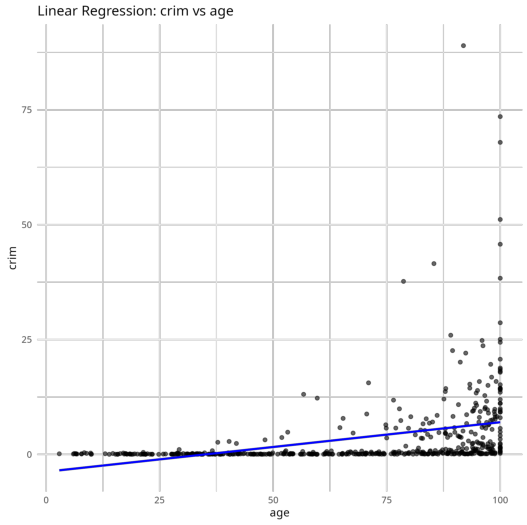
\includegraphics{hw1_files/figure-pdf/unnamed-chunk-16-1.pdf}

}

\end{figure}

\begin{verbatim}
Displaying: crim_plots/crim_vs_black.png 
\end{verbatim}

\begin{figure}[H]

{\centering 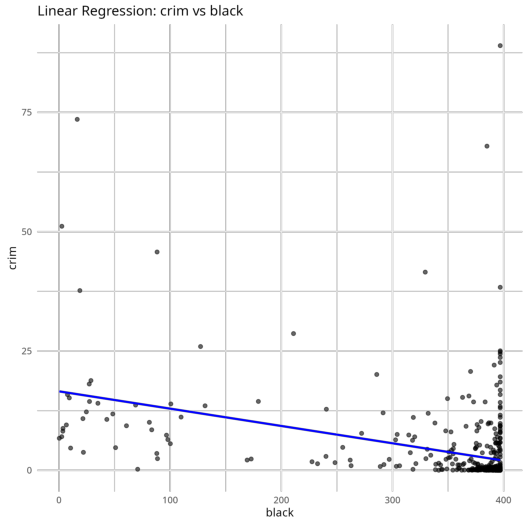
\includegraphics{hw1_files/figure-pdf/unnamed-chunk-16-2.pdf}

}

\end{figure}

\begin{verbatim}
Displaying: crim_plots/crim_vs_dis.png 
\end{verbatim}

\begin{figure}[H]

{\centering 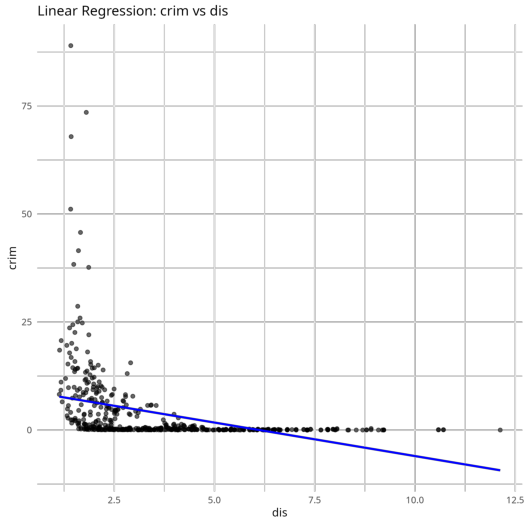
\includegraphics{hw1_files/figure-pdf/unnamed-chunk-16-3.pdf}

}

\end{figure}

\begin{verbatim}
Displaying: crim_plots/crim_vs_indus.png 
\end{verbatim}

\begin{figure}[H]

{\centering 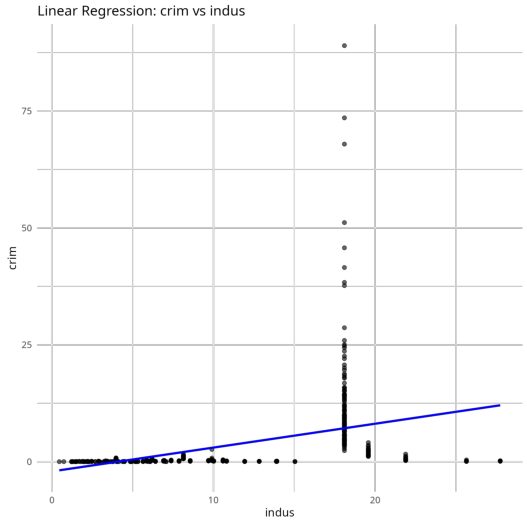
\includegraphics{hw1_files/figure-pdf/unnamed-chunk-16-4.pdf}

}

\end{figure}

\begin{verbatim}
Displaying: crim_plots/crim_vs_lstat.png 
\end{verbatim}

\begin{figure}[H]

{\centering 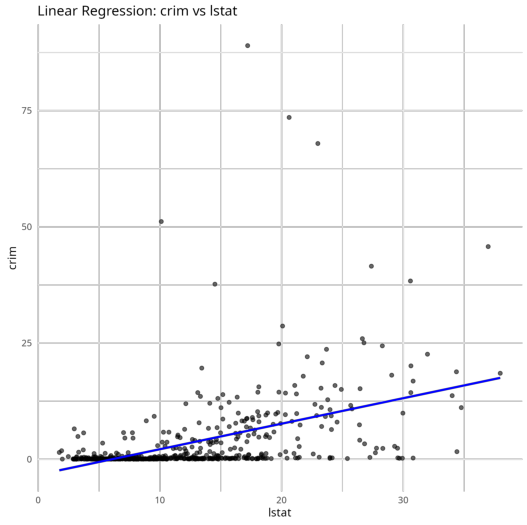
\includegraphics{hw1_files/figure-pdf/unnamed-chunk-16-5.pdf}

}

\end{figure}

\begin{verbatim}
Displaying: crim_plots/crim_vs_medv.png 
\end{verbatim}

\begin{figure}[H]

{\centering 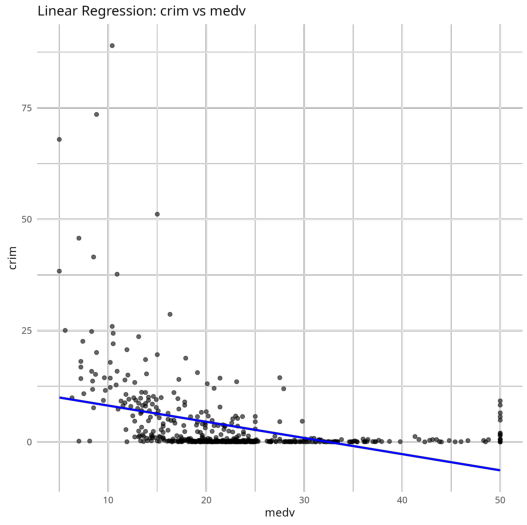
\includegraphics{hw1_files/figure-pdf/unnamed-chunk-16-6.pdf}

}

\end{figure}

\begin{verbatim}
Displaying: crim_plots/crim_vs_nox.png 
\end{verbatim}

\begin{figure}[H]

{\centering 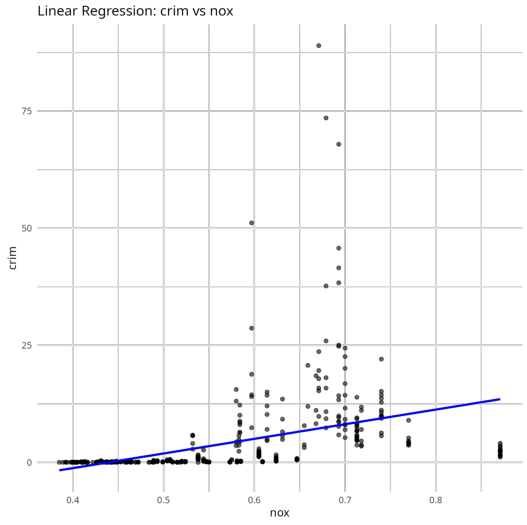
\includegraphics{hw1_files/figure-pdf/unnamed-chunk-16-7.pdf}

}

\end{figure}

\begin{verbatim}
Displaying: crim_plots/crim_vs_ptratio.png 
\end{verbatim}

\begin{figure}[H]

{\centering 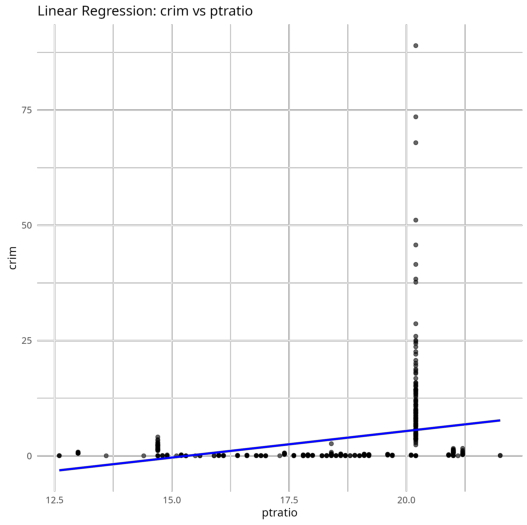
\includegraphics{hw1_files/figure-pdf/unnamed-chunk-16-8.pdf}

}

\end{figure}

\begin{verbatim}
Displaying: crim_plots/crim_vs_rad.png 
\end{verbatim}

\begin{figure}[H]

{\centering 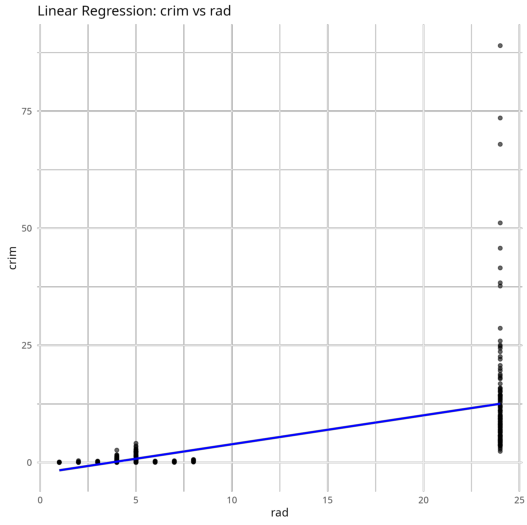
\includegraphics{hw1_files/figure-pdf/unnamed-chunk-16-9.pdf}

}

\end{figure}

\begin{verbatim}
Displaying: crim_plots/crim_vs_rm.png 
\end{verbatim}

\begin{figure}[H]

{\centering 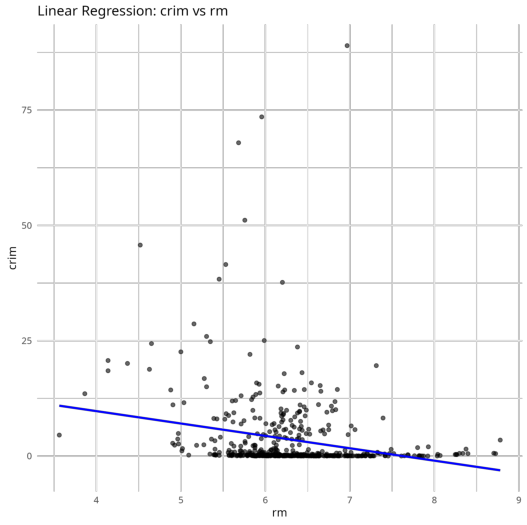
\includegraphics{hw1_files/figure-pdf/unnamed-chunk-16-10.pdf}

}

\end{figure}

\begin{verbatim}
Displaying: crim_plots/crim_vs_tax.png 
\end{verbatim}

\begin{figure}[H]

{\centering 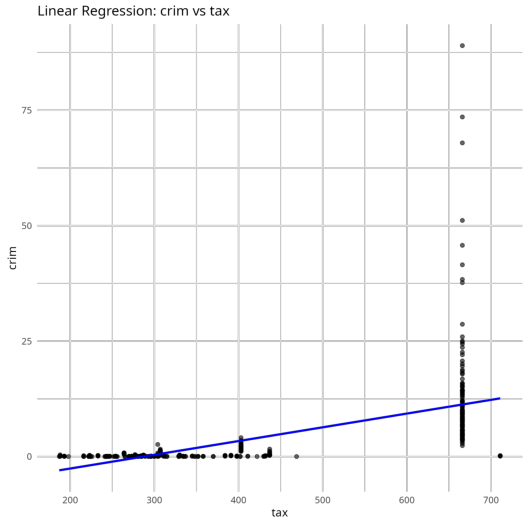
\includegraphics{hw1_files/figure-pdf/unnamed-chunk-16-11.pdf}

}

\end{figure}

\begin{verbatim}
Displaying: crim_plots/crim_vs_zn.png 
\end{verbatim}

\begin{figure}[H]

{\centering 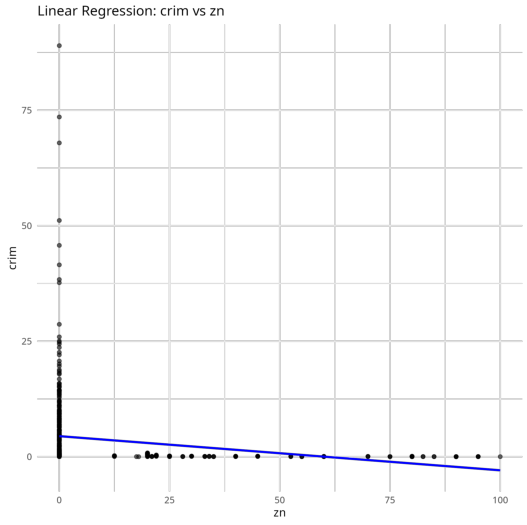
\includegraphics{hw1_files/figure-pdf/unnamed-chunk-16-12.pdf}

}

\end{figure}

zn: Negative correlation indicates that a higher proportion of
large-scale residential land is associated with lower crime rates.
indus: Positive correlation, the higher the proportion of industrial
land, the higher the crime rate. nox: Strong positive correlation
indicates a significant correlation between air pollution level (nitric
oxide concentration) and crime rate. rm: Negative correlation, the more
average rooms there are, the lower the crime rate. age: Positive
correlation, the higher the proportion of old houses, the slightly
higher the crime rate. dis: Negative correlation, the farther away from
the employment center, the lower the crime rate. rad: Strong positive
correlation, the higher the radiation radius index (indicating high
accessibility), the higher the crime rate. tax: Positive correlation,
the higher the property tax rate, the slightly higher the crime rate.
ptratio: Positive correlation, the higher the student teacher ratio, the
higher the crime rate. black: Negative correlation indicates that areas
with a higher proportion of black people have lower crime rates.

In all of models, there is a statistically significant association
between the preditctor and response.

(b)

\begin{Shaded}
\begin{Highlighting}[]
\FunctionTok{library}\NormalTok{(MASS)}
\FunctionTok{data}\NormalTok{(Boston)}

\NormalTok{multi\_model }\OtherTok{\textless{}{-}} \FunctionTok{lm}\NormalTok{(crim }\SpecialCharTok{\textasciitilde{}}\NormalTok{ ., }\AttributeTok{data =}\NormalTok{ Boston)}

\NormalTok{summary\_multi\_model }\OtherTok{\textless{}{-}} \FunctionTok{summary}\NormalTok{(multi\_model)}
\FunctionTok{print}\NormalTok{(summary\_multi\_model)}
\end{Highlighting}
\end{Shaded}

\begin{verbatim}

Call:
lm(formula = crim ~ ., data = Boston)

Residuals:
   Min     1Q Median     3Q    Max 
-9.924 -2.120 -0.353  1.019 75.051 

Coefficients:
              Estimate Std. Error t value Pr(>|t|)    
(Intercept)  17.033228   7.234903   2.354 0.018949 *  
zn            0.044855   0.018734   2.394 0.017025 *  
indus        -0.063855   0.083407  -0.766 0.444294    
chas         -0.749134   1.180147  -0.635 0.525867    
nox         -10.313535   5.275536  -1.955 0.051152 .  
rm            0.430131   0.612830   0.702 0.483089    
age           0.001452   0.017925   0.081 0.935488    
dis          -0.987176   0.281817  -3.503 0.000502 ***
rad           0.588209   0.088049   6.680 6.46e-11 ***
tax          -0.003780   0.005156  -0.733 0.463793    
ptratio      -0.271081   0.186450  -1.454 0.146611    
black        -0.007538   0.003673  -2.052 0.040702 *  
lstat         0.126211   0.075725   1.667 0.096208 .  
medv         -0.198887   0.060516  -3.287 0.001087 ** 
---
Signif. codes:  0 '***' 0.001 '**' 0.01 '*' 0.05 '.' 0.1 ' ' 1

Residual standard error: 6.439 on 492 degrees of freedom
Multiple R-squared:  0.454, Adjusted R-squared:  0.4396 
F-statistic: 31.47 on 13 and 492 DF,  p-value: < 2.2e-16
\end{verbatim}

\begin{Shaded}
\begin{Highlighting}[]
\NormalTok{multi\_reg\_results }\OtherTok{\textless{}{-}} \FunctionTok{data.frame}\NormalTok{(}
  \AttributeTok{Predictor =} \FunctionTok{rownames}\NormalTok{(summary\_multi\_model}\SpecialCharTok{$}\NormalTok{coefficients),}
  \AttributeTok{Coefficient =}\NormalTok{ summary\_multi\_model}\SpecialCharTok{$}\NormalTok{coefficients[, }\DecValTok{1}\NormalTok{],}
  \AttributeTok{p\_Value =}\NormalTok{ summary\_multi\_model}\SpecialCharTok{$}\NormalTok{coefficients[, }\DecValTok{4}\NormalTok{]}
\NormalTok{)}

\NormalTok{significant\_vars }\OtherTok{\textless{}{-}}\NormalTok{ multi\_reg\_results}\SpecialCharTok{$}\NormalTok{Predictor[multi\_reg\_results}\SpecialCharTok{$}\NormalTok{p\_Value }\SpecialCharTok{\textless{}} \FloatTok{0.05}\NormalTok{]}

\FunctionTok{print}\NormalTok{(}\StringTok{"Significant Predictors:"}\NormalTok{)}
\end{Highlighting}
\end{Shaded}

\begin{verbatim}
[1] "Significant Predictors:"
\end{verbatim}

\begin{Shaded}
\begin{Highlighting}[]
\FunctionTok{print}\NormalTok{(significant\_vars)}
\end{Highlighting}
\end{Shaded}

\begin{verbatim}
[1] "(Intercept)" "zn"          "dis"         "rad"         "black"      
[6] "medv"       
\end{verbatim}

zn:The regression coefficient is 0.0448, indicating a positive
correlation between the proportion of large-scale residential land and
the crime rate.dis:The regression coefficient is -0.9872, indicating
that the further away from the employment center, the lower the crime
rate (negative correlation).rad:The regression coefficient is 0.5882,
and the higher the radiation index, the higher the crime rate (positive
correlation).black:The regression coefficient is -0.0075, indicating a
negative correlation between the proportion of black people and the
crime rate.medv:The regression coefficient is -0.1988, indicating that
the higher the median housing price, the lower the crime rate (negative
correlation).

The p-values of Indus, Chas, NOx, RM, Age, Tax, and PTRatio are greater
than 0.05, therefore they cannot be considered significantly correlated
with crime rates.

The p-values of zn, dis, rad, black, medv are less than 0.05, so they
can reject the null hypothesis.

(c)

\begin{Shaded}
\begin{Highlighting}[]
\CommentTok{\# Merge results from (a) and (b)}
\NormalTok{merged\_results }\OtherTok{\textless{}{-}} \FunctionTok{merge}\NormalTok{(}
\NormalTok{  simple\_reg\_results,}
\NormalTok{  multi\_reg\_results,}
  \AttributeTok{by.x =} \StringTok{"Predictor"}\NormalTok{,}
  \AttributeTok{by.y =} \StringTok{"Predictor"}\NormalTok{,}
  \AttributeTok{suffixes =} \FunctionTok{c}\NormalTok{(}\StringTok{"\_Simple"}\NormalTok{, }\StringTok{"\_Multiple"}\NormalTok{)}
\NormalTok{)}

\FunctionTok{ggplot}\NormalTok{(merged\_results, }\FunctionTok{aes}\NormalTok{(}\AttributeTok{x =}\NormalTok{ Coefficient\_Simple, }\AttributeTok{y =}\NormalTok{ Coefficient\_Multiple)) }\SpecialCharTok{+}
  \FunctionTok{geom\_point}\NormalTok{(}\AttributeTok{size =} \DecValTok{2}\NormalTok{) }\SpecialCharTok{+}
  \FunctionTok{geom\_abline}\NormalTok{(}\AttributeTok{intercept =} \DecValTok{0}\NormalTok{, }\AttributeTok{slope =} \DecValTok{1}\NormalTok{, }\AttributeTok{color =} \StringTok{"red"}\NormalTok{, }\AttributeTok{linetype =} \StringTok{"dashed"}\NormalTok{) }\SpecialCharTok{+}
  \FunctionTok{ggtitle}\NormalTok{(}\StringTok{"Comparison of Coefficients: Simple vs. Multiple Regression"}\NormalTok{) }\SpecialCharTok{+}
  \FunctionTok{xlab}\NormalTok{(}\StringTok{"Simple Regression Coefficients"}\NormalTok{) }\SpecialCharTok{+}
  \FunctionTok{ylab}\NormalTok{(}\StringTok{"Multiple Regression Coefficients"}\NormalTok{) }\SpecialCharTok{+}
  \FunctionTok{theme\_minimal}\NormalTok{()}
\end{Highlighting}
\end{Shaded}

\begin{figure}[H]

{\centering 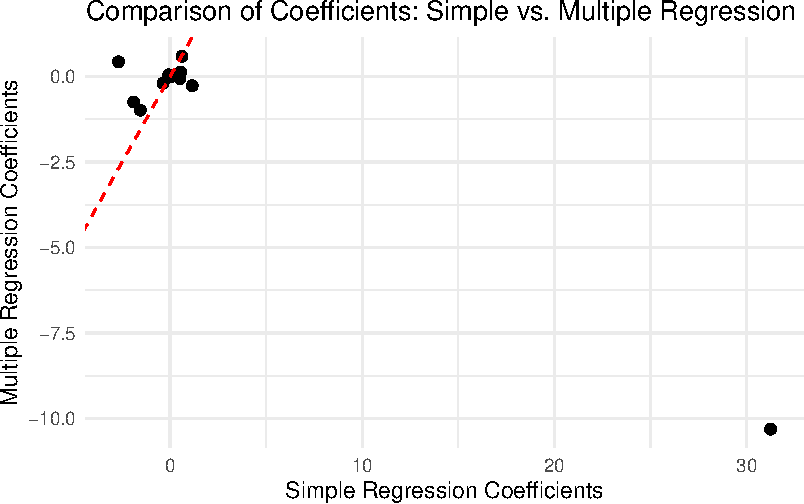
\includegraphics{hw1_files/figure-pdf/unnamed-chunk-18-1.pdf}

}

\end{figure}

(d)

\begin{Shaded}
\begin{Highlighting}[]
\NormalTok{nonlinear\_results }\OtherTok{\textless{}{-}} \FunctionTok{data.frame}\NormalTok{(}\AttributeTok{Predictor =} \FunctionTok{character}\NormalTok{(), }\AttributeTok{Linear\_P =} \FunctionTok{numeric}\NormalTok{(), }\AttributeTok{Quadratic\_P =} \FunctionTok{numeric}\NormalTok{(), }\AttributeTok{Cubic\_P =} \FunctionTok{numeric}\NormalTok{())}

\ControlFlowTok{for}\NormalTok{ (predictor }\ControlFlowTok{in} \FunctionTok{colnames}\NormalTok{(Boston)[}\SpecialCharTok{{-}}\DecValTok{1}\NormalTok{]) \{}
\NormalTok{  model }\OtherTok{\textless{}{-}} \FunctionTok{lm}\NormalTok{(crim }\SpecialCharTok{\textasciitilde{}}\NormalTok{ Boston[[predictor]] }\SpecialCharTok{+} \FunctionTok{I}\NormalTok{(Boston[[predictor]]}\SpecialCharTok{\^{}}\DecValTok{2}\NormalTok{) }\SpecialCharTok{+} \FunctionTok{I}\NormalTok{(Boston[[predictor]]}\SpecialCharTok{\^{}}\DecValTok{3}\NormalTok{), }\AttributeTok{data =}\NormalTok{ Boston)}
\NormalTok{  summary\_model }\OtherTok{\textless{}{-}} \FunctionTok{summary}\NormalTok{(model)}

\NormalTok{  coef\_matrix }\OtherTok{\textless{}{-}} \FunctionTok{coef}\NormalTok{(summary\_model)}
  \ControlFlowTok{if}\NormalTok{ (}\FunctionTok{nrow}\NormalTok{(coef\_matrix) }\SpecialCharTok{\textgreater{}=} \DecValTok{4}\NormalTok{) \{  }
\NormalTok{    nonlinear\_results }\OtherTok{\textless{}{-}} \FunctionTok{rbind}\NormalTok{(nonlinear\_results, }\FunctionTok{data.frame}\NormalTok{(}
      \AttributeTok{Predictor =}\NormalTok{ predictor,}
      \AttributeTok{Linear\_P =}\NormalTok{ coef\_matrix[}\DecValTok{2}\NormalTok{, }\DecValTok{4}\NormalTok{],       }
      \AttributeTok{Quadratic\_P =}\NormalTok{ coef\_matrix[}\DecValTok{3}\NormalTok{, }\DecValTok{4}\NormalTok{],    }
      \AttributeTok{Cubic\_P =}\NormalTok{ coef\_matrix[}\DecValTok{4}\NormalTok{, }\DecValTok{4}\NormalTok{]       }
\NormalTok{    ))}
\NormalTok{  \} }\ControlFlowTok{else}\NormalTok{ \{}
 
\NormalTok{    nonlinear\_results }\OtherTok{\textless{}{-}} \FunctionTok{rbind}\NormalTok{(nonlinear\_results, }\FunctionTok{data.frame}\NormalTok{(}
      \AttributeTok{Predictor =}\NormalTok{ predictor,}
      \AttributeTok{Linear\_P =} \FunctionTok{ifelse}\NormalTok{(}\FunctionTok{nrow}\NormalTok{(coef\_matrix) }\SpecialCharTok{\textgreater{}=} \DecValTok{2}\NormalTok{, coef\_matrix[}\DecValTok{2}\NormalTok{, }\DecValTok{4}\NormalTok{], }\ConstantTok{NA}\NormalTok{),}
      \AttributeTok{Quadratic\_P =} \FunctionTok{ifelse}\NormalTok{(}\FunctionTok{nrow}\NormalTok{(coef\_matrix) }\SpecialCharTok{\textgreater{}=} \DecValTok{3}\NormalTok{, coef\_matrix[}\DecValTok{3}\NormalTok{, }\DecValTok{4}\NormalTok{], }\ConstantTok{NA}\NormalTok{),}
      \AttributeTok{Cubic\_P =} \ConstantTok{NA}
\NormalTok{    ))}
\NormalTok{  \}}
\NormalTok{\}}
 
\NormalTok{significant\_nonlinear }\OtherTok{\textless{}{-}} \FunctionTok{subset}\NormalTok{(nonlinear\_results, Quadratic\_P }\SpecialCharTok{\textless{}} \FloatTok{0.05} \SpecialCharTok{|}\NormalTok{ Cubic\_P }\SpecialCharTok{\textless{}} \FloatTok{0.05}\NormalTok{, }\AttributeTok{select =} \FunctionTok{c}\NormalTok{(Predictor, Quadratic\_P, Cubic\_P))}
\FunctionTok{print}\NormalTok{(}\StringTok{"Significant Non{-}Linear Predictors:"}\NormalTok{)}
\end{Highlighting}
\end{Shaded}

\begin{verbatim}
[1] "Significant Non-Linear Predictors:"
\end{verbatim}

\begin{Shaded}
\begin{Highlighting}[]
\FunctionTok{print}\NormalTok{(significant\_nonlinear)}
\end{Highlighting}
\end{Shaded}

\begin{verbatim}
   Predictor  Quadratic_P      Cubic_P
2      indus 3.420187e-10 1.196405e-12
4        nox 6.811300e-15 6.961110e-16
6        age 4.737733e-02 6.679915e-03
7        dis 4.941214e-12 1.088832e-08
10   ptratio 4.119552e-03 6.300514e-03
13      medv 3.260523e-18 1.046510e-12
\end{verbatim}

\begin{Shaded}
\begin{Highlighting}[]
\FunctionTok{library}\NormalTok{(ggplot2)}
\ControlFlowTok{for}\NormalTok{ (predictor }\ControlFlowTok{in}\NormalTok{ significant\_nonlinear}\SpecialCharTok{$}\NormalTok{Predictor) \{}
\NormalTok{  p }\OtherTok{\textless{}{-}} \FunctionTok{ggplot}\NormalTok{(Boston, }\FunctionTok{aes\_string}\NormalTok{(}\AttributeTok{x =}\NormalTok{ predictor, }\AttributeTok{y =} \StringTok{"crim"}\NormalTok{)) }\SpecialCharTok{+}
    \FunctionTok{geom\_point}\NormalTok{(}\AttributeTok{alpha =} \FloatTok{0.6}\NormalTok{) }\SpecialCharTok{+}
    \FunctionTok{geom\_smooth}\NormalTok{(}\AttributeTok{method =} \StringTok{"lm"}\NormalTok{, }\AttributeTok{formula =}\NormalTok{ y }\SpecialCharTok{\textasciitilde{}} \FunctionTok{poly}\NormalTok{(x, }\DecValTok{3}\NormalTok{), }\AttributeTok{color =} \StringTok{"blue"}\NormalTok{, }\AttributeTok{se =} \ConstantTok{FALSE}\NormalTok{) }\SpecialCharTok{+}
    \FunctionTok{ggtitle}\NormalTok{(}\FunctionTok{paste}\NormalTok{(}\StringTok{"Non{-}Linear Relationship (Cubic): crim vs"}\NormalTok{, predictor)) }\SpecialCharTok{+}
    \FunctionTok{xlab}\NormalTok{(predictor) }\SpecialCharTok{+}
    \FunctionTok{ylab}\NormalTok{(}\StringTok{"crim"}\NormalTok{) }\SpecialCharTok{+}
    \FunctionTok{theme\_minimal}\NormalTok{()}
  
  \FunctionTok{print}\NormalTok{(p)}
\NormalTok{\}}
\end{Highlighting}
\end{Shaded}

\begin{verbatim}
Warning: `aes_string()` was deprecated in ggplot2 3.0.0.
i Please use tidy evaluation idioms with `aes()`.
i See also `vignette("ggplot2-in-packages")` for more information.
\end{verbatim}

\begin{figure}[H]

{\centering 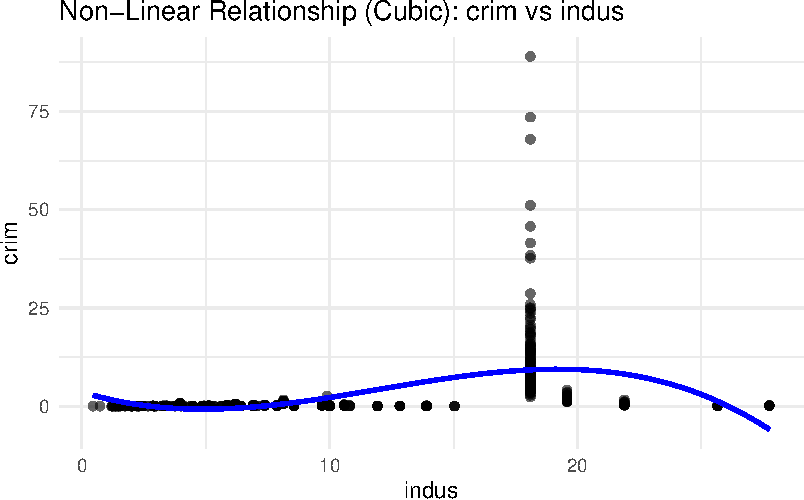
\includegraphics{hw1_files/figure-pdf/unnamed-chunk-20-1.pdf}

}

\end{figure}

\begin{figure}[H]

{\centering 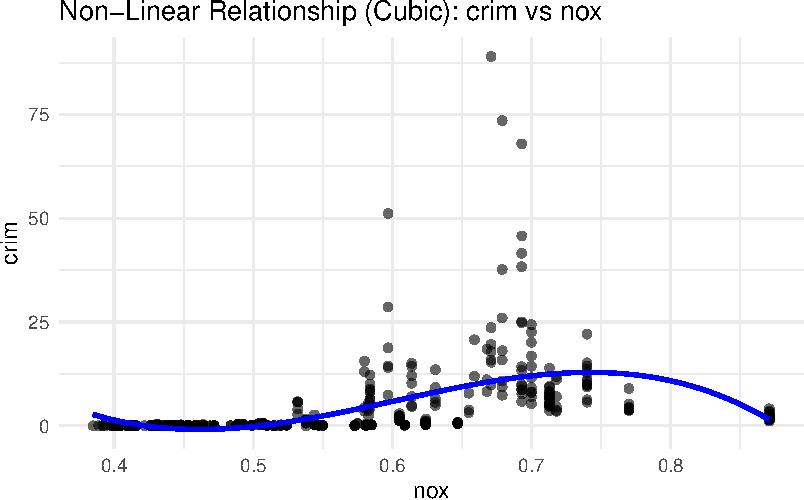
\includegraphics{hw1_files/figure-pdf/unnamed-chunk-20-2.pdf}

}

\end{figure}

\begin{figure}[H]

{\centering 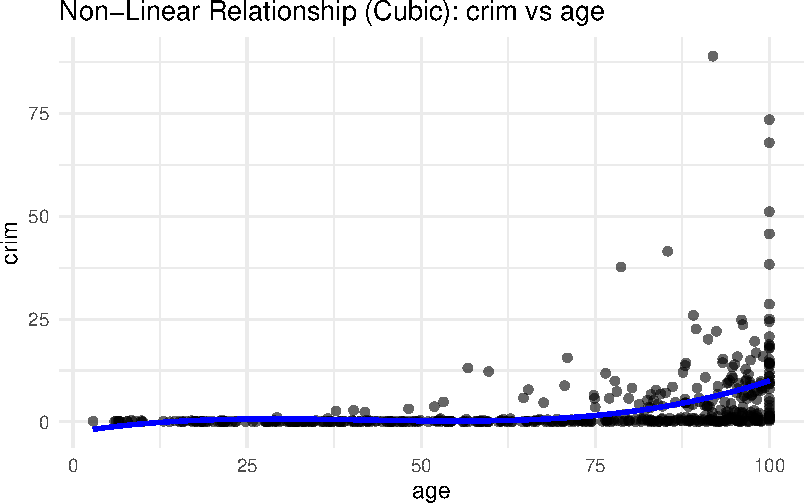
\includegraphics{hw1_files/figure-pdf/unnamed-chunk-20-3.pdf}

}

\end{figure}

\begin{figure}[H]

{\centering 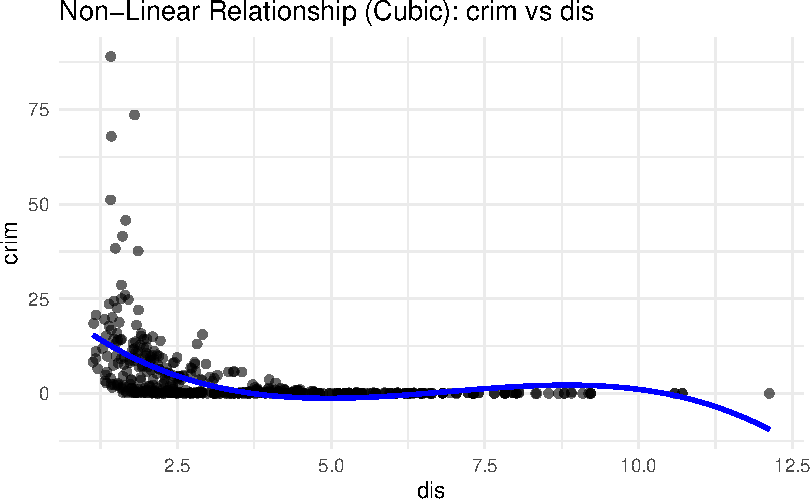
\includegraphics{hw1_files/figure-pdf/unnamed-chunk-20-4.pdf}

}

\end{figure}

\begin{figure}[H]

{\centering 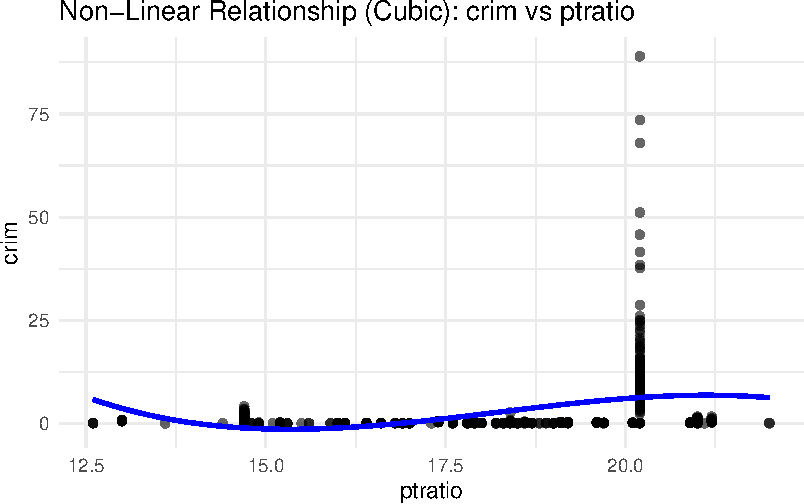
\includegraphics{hw1_files/figure-pdf/unnamed-chunk-20-5.pdf}

}

\end{figure}

\begin{figure}[H]

{\centering 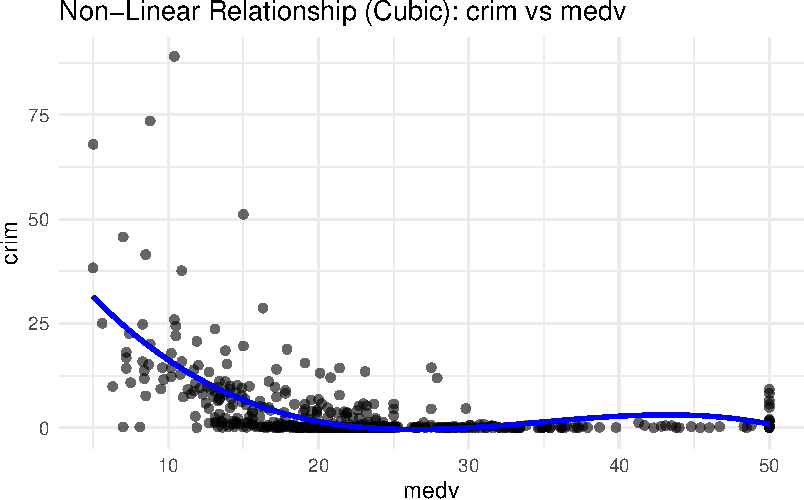
\includegraphics{hw1_files/figure-pdf/unnamed-chunk-20-6.pdf}

}

\end{figure}

The relationship between these variables (Indus, NOx, age,dis, ptratio
and medv.) and Crimea is not a simple linear relationship, but a more
complex curve relationship (including U-shaped trends or other nonlinear
patterns).

\hypertarget{bonus-question-20-pts}{%
\subsection{Bonus question (20\% pts)}\label{bonus-question-20-pts}}

For multiple linear regression, show that \(R^2\) is equal to the
correlation between the response vector
\(\mathbf{y} = (y_1, \ldots, y_n)^T\) and the fitted values
\(\hat{\mathbf{y}} = (\hat y_1, \ldots, \hat y_n)^T\). That is \[
R^2 = 1 - \frac{\text{RSS}}{\text{TSS}} = [\operatorname{Cor}(\mathbf{y}, \hat{\mathbf{y}})]^2.
\]

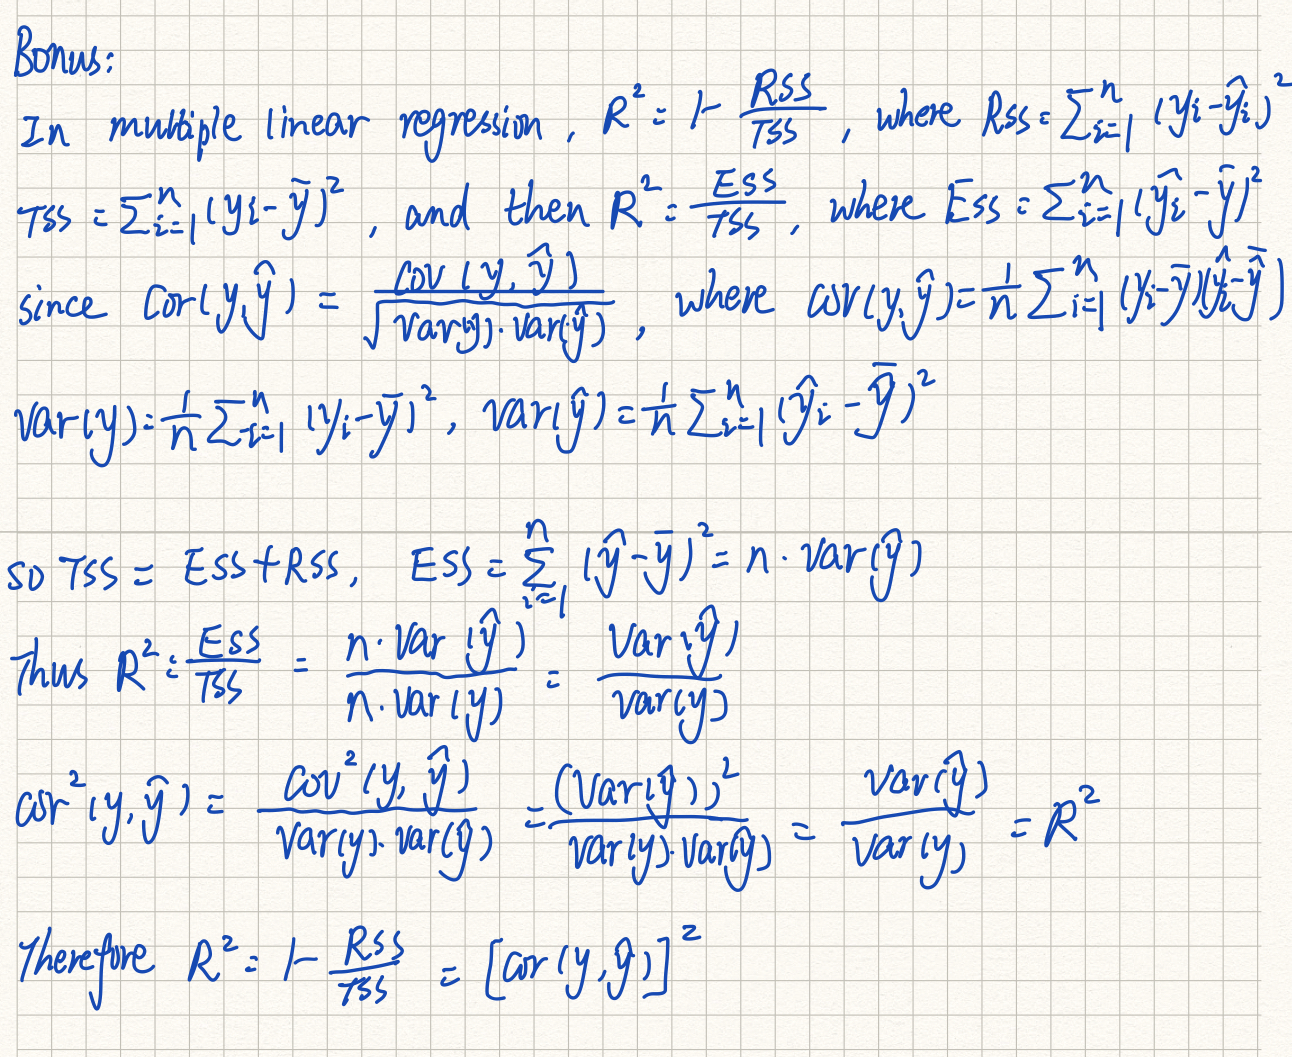
\includegraphics{images/clipboard-1942909937.jpeg}



\end{document}
